% Template:     Informe/Reporte LaTeX
% Documento:    Archivo principal
% Versión:      4.3.6 (30/07/2017)
% Codificación: UTF-8
%
% Autor: Pablo Pizarro R.
%        Facultad de Ciencias Físicas y Matemáticas
%        Universidad de Chile
%        pablo.pizarro@ing.uchile.cl, ppizarror.com
%
% Manual template: [http://latex.ppizarror.com/Template-Informe/]
% Licencia MIT:    [https://opensource.org/licenses/MIT/]

% CREACIÓN DEL DOCUMENTO
\documentclass[letterpaper,11pt]{article} % Articulo tamaño carta, 11pt
\usepackage[utf8]{inputenc} % Codificación UTF-8

% INFORMACIÓN DEL DOCUMENTO
\def\titulodelinforme {Informe de Práctica Profesional I}
\def\temaatratar {Web Intelligence Centre}

\def\autordeldocumento {Gabriel Iturra Bocaz}
\def\nombredelcurso {Práctica Profesional I}
\def\codigodelcurso {CC-4901}

\def\nombreuniversidad {Universidad de Chile}
\def\nombrefacultad {Facultad de Ciencias Físicas y Matemáticas}
\def\departamentouniversidad {Departamento de Ciencias de Computación}
\def\imagendepartamento {departamentos/dcc}
\def\imagendepartamentoescala {0.2}
\def\localizacionuniversidad {Santiago, Chile}

% INTEGRANTES, PROFESORES Y FECHAS
\def\tablaintegrantes {
\begin{minipage}{0.976\textwidth}
\begin{flushright}\begin{tabular}{ll}
	Nombre:
		& \begin{tabular}[t]{@{}l@{}}
			Gabriel Iturra Bocaz\\
		\end{tabular} \\
	Carrera:
		& \begin{tabular}[t]{@{}l@{}}
			Ingeniería Civil Industrial\\
		\end{tabular} \\
	Rut:
		& \begin{tabular}[t]{@{}l@{}}
			18.214.940-3 \\
		\end{tabular} \\
	Correo:
		& \begin{tabular}[t]{@{}l@{}}
			gabrieliturrab@ug.uchile.cl \\
		\end{tabular} \\
	Profesor:
		& \begin{tabular}[t]{@{}l@{}}
			Alexandre Bergel \\
		\end{tabular} \\
	\multicolumn{2}{l}{Fecha de realización: 3 al 31 de Enero de 2017} \\
	\multicolumn{2}{l}{Fecha de entrega: 1 de Septiembre de 2017} \\
	\multicolumn{2}{l}{\localizacionuniversidad}
\end{tabular}\end{flushright}
\end{minipage}
}

% CONFIGURACIONES
% Template:     Informe/Reporte LaTeX
% Documento:    Configuraciones del template
% Versión:      4.3.6 (30/07/2017)
% Codificación: UTF-8
%
% Autor: Pablo Pizarro R.
%        Facultad de Ciencias Físicas y Matemáticas
%        Universidad de Chile
%        pablo.pizarro@ing.uchile.cl, ppizarror.com
%
% Manual template: [http://latex.ppizarror.com/Template-Informe/]
% Licencia MIT:    [https://opensource.org/licenses/MIT/]

% CONFIGURACIONES GENERALES
\def\addemptypagetwosides {false}  % Añade pags. en blanco al imprimir a 2 caras
\def\anumsecaddtocounter {false}   % Función para insertar títulos anum. aumenta contador
\def\defaultinterline {1.0}        % Interlineado por defecto [pt]
\def\defaultnewlinesize {11.0}     % Tamaño del salto de línea [pt]
\def\fontdocument {lmodern}        % Tipografía (lmodern,arial,helvet)
\def\numberedequation {true}       % Ecuaciones con \insert... numeradas
\def\pointdecimal {false}          % Decimales con punto en vez de coma
\def\romanpageuppercase {false}    % Páginas en número romano en mayúsculas
\def\showdotontitles {true}        % Punto al final de cada número de título/sub(sub)título
\def\tablepadding {1.0}            % Ancho de celda de las tablas

% ESTILO PORTADA Y HEADER-FOOTER
\def\hfstyle {style1}              % Estilo del header-footer (6 estilos distintos)
\def\portraitstyle {style2}        % Estilo de la portada (4 estilos distintos)

% MÁRGENES DE PÁGINA
\def\firstpagemargintop {3.8}      % Margen superior página portada [cm]
\def\pagemarginbottom {2.7}        % Margen inferior página [cm]
\def\pagemarginleft {2.54}         % Margen izquierdo página [cm]
\def\pagemarginright {2.54}        % Margen derecho página [cm]
\def\pagemargintop {3.0}           % Margen superior página [cm]

% CONFIGURACIÓN DE LAS LEYENDAS - CAPTION
\def\captionlessmarginimage {0.1}  % Margen sup/inf de fig si no hay leyenda [cm]
\def\captionlrmargin {2.0}         % Márgenes izq/der de la leyenda [cm]
\def\captionalignment {justified}  % Alineación leyenda: justified,centered,left,right
\def\captiontbmarginfigure {9.35}  % Margen sup/inf de la leyenda en figuras [pt]
\def\captiontbmargintable {7.0}    % Margen sup/inf de la leyenda en tablas [pt]
\def\captiontextbold {false}       % Etiquetas (Código,Figura,Tabla) en negrita
\def\codecaptiontop {true}         % Leyenda arriba del código fuente
\def\figurecaptiontop {false}      % Leyenda arriba de las imágenes
\def\showsectiononcaption {false}  % Muestra el número de sección en las leyendas
\def\tablecaptiontop {true}        % Leyenda arriba de las tablas

% CONFIGURACIÓN DEL ÍNDICE
\def\indexdepth {3}                % Profundidad máxima del índice
\def\indextitlemargin {7.0}        % Margen título en índice \insertindextitle [pt]
\def\showdotonobjectindex {false}  % Punto en cada número de figura, tabla o código
\def\showdotpagenumindex {true}    % Muestra puntos entre objeto y número de página
\def\showindex {true}              % Muestra el índice
\def\showindexofcode {true}        % Muestra la lista de códigos fuente
\def\showindexofcontents {true}    % Muestra la lista de contenidos
\def\showindexoffigures {true}     % Muestra la lista de figuras
\def\showindexoftables {true}      % Muestra la lista de tablas

% CONFIGURACIÓN DE LOS COLORES DEL DOCUMENTO
\def\captioncolor {black}          % Color de la etiqueta (Código,Figura,Tabla)
\def\captiontextcolor {black}      % Color de la leyenda
\def\citecolor {black}             % Color del número de las referencias o citas
\def\highlightcolor {yellow}       % Color del subrayado con \hl
\def\indextitlecolor {black}       % Color de los títulos del índice
\def\linkcolor {black}             % Color de los links del doc.
\def\maintextcolor {black}         % Color principal del texto
\def\portraittitlecolor {black}    % Color de los títulos de la portada
\def\showborderonlinks {false}     % Color de un links por un recuadro de color
\def\subsubtitlecolor {black}      % Color de los sub-subtítulos
\def\subtitlecolor {black}         % Color de los subtítulos
\def\tablelinecolor {black}        % Color de las líneas de las tablas
\def\titlecolor {black}            % Color de los títulos
\def\urlcolor {magenta}            % Color de los enlaces web (\url,\href)

% CONFIGURACIÓN DE FIGURAS
\def\defaultimagefolder {images/}  % Carpeta raíz de las imágenes
\def\marginbottomimages {-0.2}     % Margen inferior figura [cm]
\def\marginfloatimages {-13.0}     % Margen sup. fig. float \insertimageleft/right [pt]
\def\margintopimages {0.0}         % Margen superior figura [cm]

% ANEXO, CITAS, REFERENCIAS
\def\apaciterefsep {9}             % Separación entre referencias [pt] {apacite}
\def\appendixindepobjnum {false}    % Anexo usa número objetos de forma independiente
\def\bibtexrefsep {9}              % Separación entre referencias [pt] {bibtex}
\def\natbibrefsep {5}              % Separación entre referencias [pt] {natbib}
\def\referencenumsection {false}   % Sección de referencias numerada
\def\sectionappendixlastchar {.}   % Caracter entre el n° de la sec. de anexo y el título
\def\showappendixsecindex {false}  % Muestra el título de la sec. de anexos en el índice
\def\showappendixsectitle {false}  % Muestra el título de la sec. de anexo en el informe
\def\stylecitereferences {bibtex}  % Estilo citas y referencias (bibtex,apacite,natbib)
\def\twocolumnreferences {false}   % Referencias en dos columnas

% ESTILO Y TAMAÑO DE TÍTULOS
\def\fontsizesubsubtitle {\large}  % Tamaño sub-subtítulos
\def\fontsizesubtitle {\Large}     % Tamaño subtítulos
\def\fontsizetitle {\huge}         % Tamaño títulos
\def\fontsizetitlei {\huge}        % Tamaño títulos en el índice
\def\stylesubsubtitle {\bfseries}  % Estilo sub-subtítulos
\def\stylesubtitle {\bfseries}     % Estilo subtítulos
\def\styletitle {\bfseries}        % Estilo títulos
\def\styletitlei {\bfseries}       % Estilo títulos en el índice

% NOMBRE DE OBJETOS
\def\nameabstract {Resumen}           % Nombre del resumen-abstract
\def\nameappendixsection{Anexos}      % Nombre de la sección de anexos/apéndices
\def\nameportraitpage {Portada}       % Etiqueta página de la portada
\def\namereferences {Referencias}     % Nombre de la sección de referencias
\def\nomltappendixsection {Anexo}     % Etiqueta sección en anexo/apéndices
\def\nomltcont {Índice General} % Nombre del índice de contenidos
\def\nomltfigure {Lista de Figuras}   % Nombre del índice de la lista de figuras
\def\nomltsrc {Lista de Códigos}      % Nombre del índice de la lista de código
\def\nomlttable {Lista de Tablas}     % Nombre del índice de la lista de tablas
\def\nomltwfigure {Figura}            % Etiqueta leyenda de las figuras
\def\nomltwsrc {Código}               % Etiqueta leyenda del código fuente
\def\nomltwtable {Tabla}              % Etiqueta leyenda de las tablas

% OPCIONES DEL PDF COMPILADO
\def\cfgbookmarksopenlevel {2}     % Nivel de los marcadores a mostrar (2: subsecciones)
\def\cfgpdfbookmarkopen {true}     % Expande los marcadores hasta el nivel configurado
\def\cfgpdfcenterwindow {true}     % Centra la ventana del lector al abrir el pdf
\def\cfgpdfcopyright {}            % Establece el copyright del documento
\def\cfgpdfdisplaydoctitle {true}  % Muestra el título del informe como título del pdf
\def\cfgpdffitwindow {false}       % Ajusta la ventana del lector al tamaño del pdf
\def\cfgpdfmenubar {true}          % Muestra el menú del lector al abrir el pdf
\def\cfgpdftoolbar {true}          % Muestra la barra de herramientas del lector pdf
\def\cfgshowbookmarkmenu {true}    % Muestra el menú de los marcadores en el lector pdf


% IMPORTACIÓN DE LIBRERÍAS
% Template:     Informe/Reporte LaTeX
% Documento:    Importación de librerías
% Versión:      4.3.6 (30/07/2017)
% Codificación: UTF-8
%
% Autor: Pablo Pizarro R.
%        Facultad de Ciencias Físicas y Matemáticas
%        Universidad de Chile
%        pablo.pizarro@ing.uchile.cl, ppizarror.com
%
% Manual template: [http://latex.ppizarror.com/Template-Informe/]
% Licencia MIT:    [https://opensource.org/licenses/MIT/]

% LIBRERÍAS IMPORTANTES
\usepackage[spanish,es-nosectiondot,es-lcroman]{babel} % Idioma
\usepackage[T1]{fontenc}   % Caracteres acentuados
\usepackage{\fontdocument} % Tipografía del documento
\usepackage{ifthen}        % Manejo de condicionales

% LIBRERÍAS INDEPENDIENTES
\usepackage{amsmath}       % Librerías matemáticas
\usepackage{amssymb}       % Librerías matemáticas
\usepackage{array}         % Nuevas características a las tablas
\usepackage{bigstrut}      % Líneas horizontales en tablas
\usepackage{bm}            % Caracteres en negrita en ecuaciones
\usepackage{booktabs}      % Permite manejar elementos visuales en tablas
\usepackage{caption}       % Leyendas
\usepackage{changepage}    % Condicionales para administrar páginas
\usepackage{chngcntr}      % Añade números a las leyendas
\usepackage{colortbl}      % Administración de color en tablas
\usepackage{color}         % Colores
\usepackage{csquotes}      % Citas y comillas
\usepackage{datetime}      % Fechas
\usepackage{fancyhdr}      % Encabezados y pié de páginas
\usepackage{floatpag}      % Maneja números de páginas
\usepackage{floatrow}      % Permite adminisrar posiciones en los caption
\usepackage{gensymb}       % Simbología común
\usepackage{geometry}      % Dimensiones y geometría del documento
\usepackage{graphicx}      % Propiedades extra para los gráficos
\usepackage{lipsum}        % Permite crear textos dummy
\usepackage{listings}      % Permite añadir código fuente
\usepackage{longtable}     % Permite utilizar tablas en varias hojas
\usepackage{mathtools}     % Permite utilizar notaciones matemáticas
\usepackage{multicol}      % Múltiples columnas
\usepackage{needspace}     % Maneja los espacios en página
\usepackage{notoccite}     % Desactiva las citas en el índice
\usepackage{pdfpages}      % Permite administrar páginas en pdf
\usepackage{physics}       % Paquete de matemáticas
\usepackage{rotating}      % Permite rotación de objetos
\usepackage{sectsty}       % Cambia el estilo de los títulos
\usepackage{selinput}      % Compatibilidad con acentos
\usepackage{setspace}      % Cambia el espacio entre líneas
\usepackage{siunitx}       % Unidades del sistema internacional
\usepackage{soul}          % Permite subrayar texto
\usepackage{subfig}        % Permite agrupar imágenes
\usepackage{textcomp}      % Simbología común
\usepackage{url}           % Permite añadir enlaces
\usepackage{wasysym}       % Contiene caracteres misceláneos
\usepackage{wrapfig}       % Permite comprimir imágenes
\usepackage{xspace}        % Adminsitra espacios en párrafos y líneas

% LIBRERÍAS CON PARÁMETROS
\usepackage[makeroom]{cancel} % Cancelar términos en fórmulas
\usepackage[inline]{enumitem} % Permite enumerar ítems
\usepackage[bottom,norule,hang]{footmisc} % Estilo pié de página
\usepackage[subfigure,titles]{tocloft} % Maneja entradas en el índice
\usepackage[pdfencoding=auto,psdextra]{hyperref} % Enlaces, referencias
\usepackage[figure,table,lstlisting]{totalcount} % Contador de objetos
\usepackage[normalem]{ulem} % Permite tachar y subrayar
\usepackage[usenames,dvipsnames]{xcolor} % Paquete de colores avanzado

% LIBRERÍAS CONDICIONALES
\ifthenelse{\equal{\showdotontitles}{true}}{ % Agrega puntos a los títulos/subtítulos
	\usepackage{secdot}
	\sectiondot{subsection}
	\sectiondot{subsubsection}}{
}
\ifthenelse{\equal{\stylecitereferences}{natbib}}{ % Formato citas natbib
	\usepackage{natbib}
}{
	\ifthenelse{\equal{\stylecitereferences}{apacite}}{ % Formato citas apacite
		\usepackage{apacite}
	}{
		\ifthenelse{\equal{\stylecitereferences}{bibtex}}{ % Formato citas bibtex
		}{
		}
	}
}
\ifthenelse{\equal{\showappendixsecindex}{true}}{ % Anexos/Apéndices
	\usepackage[toc]{appendix}
}{
	\usepackage{appendix}
}

% LIBRERÍAS DEPENDIENTES
\usepackage{bookmark}      % Administración de marcadores en pdf
\usepackage{float}         % Administrador de posiciones de objetos
\usepackage{hyperxmp}      % Etiquetas opcionales para el pdf compilado
\usepackage{multirow}      % Agrega nuevas opciones a las tablas


% IMPORTACIÓN DE FUNCIONES
% Template:     Informe/Reporte LaTeX
% Documento:    Funciones del núcleo del template
% Versión:      4.3.6 (30/07/2017)
% Codificación: UTF-8
%
% Autor: Pablo Pizarro R.
%        Facultad de Ciencias Físicas y Matemáticas
%        Universidad de Chile
%        pablo.pizarro@ing.uchile.cl, ppizarror.com
%
% Manual template: [http://latex.ppizarror.com/Template-Informe/]
% Licencia MIT:    [https://opensource.org/licenses/MIT/]

\newcommand{\throwerror}[2]{
	% Lanza un mensaje de error
	% 	#1	Función del error
	%	#2	Mensaje
	\errmessage{LaTeX Error: \noexpand#1 #2 (linea \the\inputlineno)}
	\stop
}

\newcommand{\throwwarning}[1]{
	% Lanza un mensaje de advertencia
	%	#1	Mensaje
	\errmessage{LaTeX Warning: #1 (linea \the\inputlineno)}
}

\newcommand{\throwbadconfig}[3]{
	% Lanza un mensaje de error indicando mala configuración
	%	#1	Mensaje de error
	% 	#2	Configuración usada
	%	#3	Valores esperados
	\errmessage{LaTeX Warning: #1 \noexpand #2=#2. Valores esperados: #3}
	\stop
}

\newcommand{\throwbadconfigondoc}[3]{
	% Lanza un mensaje de error indicando mala configuración dentro de begin{document}
	%	#1	Mensaje de error
	% 	#2	Configuración usada
	%	#3	Valores esperados
	\errmessage{#1 \noexpand #2=#2. Valores esperados: #3}
	\stop
}

\newcommand{\checkvardefined}[1]{
	% Comprueba si una variable está definida
	%	#1	Variable
	\ifthenelse{\isundefined{#1}}{
		\errmessage{LaTeX Warning: Variable \noexpand#1 no definida}
		\stop
	}{}
}

\newcommand{\emptyvarerr}[3]{
	% Lanza un mensaje de error si una variable no ha sido definida
	% 	#1	Función del error
	%	#2	Variable
	%	#3	Mensaje
	\ifx\hfuzz#2\hfuzz
		\errmessage{LaTeX Warning: \noexpand#1 #3 (linea \the\inputlineno)}
	\fi
}

\newcommand{\setcaptionmargincm}[1]{
	% Cambiar el margen de los caption
	% 	#1	Margen en centímetros
	\captionsetup{margin=#1cm}
}

\newcommand{\setpagemargincm}[4]{
	% Cambia márgenes de las páginas [cm]
	% 	#1	Margen izquierdo
	%	#2	Margen superior
	%	#3	Margen derecho
	%	#4	Margen inferior
	\newgeometry{left=#1cm, top=#2cm, right=#3cm, bottom=#4cm}
}

\newcommand{\changemargin}[2]{
	% Cambia los márgenes del documento
	%	#1 Margen izquierdo
	%	#2 Margen derecho
	\emptyvarerr{\changemargin}{#1}{Margen izquierdo no definido}
	\emptyvarerr{\changemargin}{#2}{Margen derecho no definido}
	\list{}{\rightmargin#2\leftmargin#1}\item[]
}
\let\endchangemargin=\endlist

% Template:     Informe/Reporte LaTeX
% Documento:    Funciones para insertar elementos
% Versión:      4.3.6 (30/07/2017)
% Codificación: UTF-8
%
% Autor: Pablo Pizarro R.
%        Facultad de Ciencias Físicas y Matemáticas
%        Universidad de Chile
%        pablo.pizarro@ing.uchile.cl, ppizarror.com
%
% Manual template: [http://latex.ppizarror.com/Template-Informe/]
% Licencia MIT:    [https://opensource.org/licenses/MIT/]

\newcommand{\newp}{
	% Inserta nueva línea
	\hbadness=10000 \vspace{\defaultnewlinesize pt} \par
}

\newcommand{\newpar}[1]{
	% Insertar párrafo
	% 	#1	Párrafo
	\hbadness=10000 #1 \newp
}

\newcommand{\newparnl}[1]{
	% Insertar párrafo sin nueva línea al final
	% 	#1	Párrafo
	#1 \par
}

\newcommand{\lpow}[2]{
	% Insertar sub-índice, a_b
	% 	#1	Elemento inferior (a)
	%	#2	Elemento superior (b)
	\ensuremath{{#1}_{#2}}
}

\newcommand{\pow}[2]{
	% Insertar elevado, a^b
	% 	#1	Elemento inferior (a)
	%	#2	Elemento superior (b)
	\ensuremath{{#1}^{#2}}
}

\newcommand{\fracpartial}[2]{
	% Fracción de derivadas parciales af/ax
	% 	#1	Función a derivar (f)
	%	#2	Variable a derivar (x)
	\ensuremath{\pdv{#1}{#2}}
}

\newcommand{\fracdpartial}[2]{
	% Fracción de derivadas parciales dobles a^2f/ax^2
	% 	#1	Función a derivar (f)
	%	#2	Variable a derivar (x)
	\ensuremath{\pdv[2]{#1}{#2}}
}

\newcommand{\fracnpartial}[3]{
	% Fracción de derivadas parciales en n, a^nf/ax^n
	% 	#1	Función a derivar (f)
	%	#2	Variable a derivar (x)
	%	#3	Orden (n)
	\ensuremath{\pdv[#3]{#1}{#2}}
}

\newcommand{\fracderivat}[2]{
	% Fracción de derivadas df/dx
	% 	#1	Función a derivar (f)
	%	#2	Variable a derivar (x)
	\ensuremath{\dv{#1}{#2}}
}

\newcommand{\fracdderivat}[2]{
	% Fracción de derivadas dobles d^2/dx^2
	% 	#1	Función a derivar (f)
	%	#2	Variable a derivar (x)
	\ensuremath{\dv[2]{#1}{#2}}
}

\newcommand{\fracnderivat}[3]{
	% Fracción de derivadas en n d^nf/dx^n
	% 	#1	Función a derivar (f)
	%	#2	Variable a derivar (x)
	%	#3	Orden de la derivada (n)
	\ensuremath{\dv[#3]{#1}{#2}}
}

\newcommand{\topequal}[2]{
	% Llave superior de equivalencia
	% 	#1	Elemento a igualar
	%	#2	Igualdad
	\ensuremath{\overbrace{#1}^{\mathclap{#2}}}
}

\newcommand{\underequal}[2]{
	% Llave inferior de equivalencia
	% 	#1	Elemento a igualar
	%	#2	Igualdad
	\ensuremath{\underbrace{#1}_{\mathclap{#2}}}
}

\newcommand{\topsequal}[2]{
	% Rectángulo superior de equivalencia
	% 	#1	Elemento a igualar
	%	#2	Igualdad
	\ensuremath{\overbracket{#1}^{\mathclap{#2}}}
}

\newcommand{\undersequal}[2]{
	% Rectángulo inferior de equivalencia
	% 	#1	Elemento a igualar
	%	#2	Igualdad
	\ensuremath{\underbracket{#1}_{\mathclap{#2}}}
}

\newcommand{\itemresize}[2]{
	% Redimensiona un ítem en textwidth
	% 	#1	Tamaño del nuevo objeto (En textwidth)
	%	#2	Objeto a redimensionar
	\emptyvarerr{\itemresize}{#1}{Tamano del nuevo objeto no definido}
	\emptyvarerr{\itemresize}{#2}{Objeto a redimensionar no definido}
	\resizebox{#1\textwidth}{!}{#2}
}

\newcommand{\insertemptypage}{
	% Crea una página vacía
	\newpage
	\setcounter{templatepagecounter}{\thepage}
	\pagenumbering{gobble}
	\null
	\thispagestyle{empty}
	\newpage
	\pagenumbering{arabic}
	\setcounter{page}{\thetemplatepagecounter}
}

% Inserta un texto entre comillas
\newcommand{\quotes}[1]{\enquote*{#1}}

% Inserta un email con un link cliqueable
\newcommand{\insertemail}[1]{\href{mailto:#1}{\texttt{#1}}}

% Template:     Informe/Reporte LaTeX
% Documento:    Funciones para insertar ecuaciones
% Versión:      4.3.6 (30/07/2017)
% Codificación: UTF-8
%
% Autor: Pablo Pizarro R.
%        Facultad de Ciencias Físicas y Matemáticas
%        Universidad de Chile
%        pablo.pizarro@ing.uchile.cl, ppizarror.com
%
% Manual template: [http://latex.ppizarror.com/Template-Informe/]
% Licencia MIT:    [https://opensource.org/licenses/MIT/]

\newcommand{\equationresize}[2]{
	% Redimensiona una ecuación en textwidth
	% 	#1	Tamaño del nuevo objeto (En textwidth)
	%	#2	Ecuación a redimensionar
	\emptyvarerr{\equationresize}{#1}{Dimension no definida}
	\emptyvarerr{\equationresize}{#2}{Ecuacion a redimensionar no definida}
	\resizebox{#1\textwidth}{!}{$#2$}
}

\newcommand{\insertequation}[2][]{
	% Insertar una ecuación
	% 	#1	Label (opcional)
	%	#2	Ecuación
	\emptyvarerr{\insertequation}{#2}{Ecuacion no definida}
	\ifthenelse{\equal{\numberedequation}{true}}{
		\vspace{-0.1cm}
		\begin{equation}
			\text{#1} #2
		\end{equation}
		\vspace{-0.26cm}
	}{
		\ifx\hfuzz#1\hfuzz
		\else
			\throwwarning{Label invalido en ecuacion sin numero}
		\fi
		\insertequationanum{#2}
	}
}

\newcommand{\insertequationanum}[1]{
	% Insertar una ecuación sin número
	%	#1	Ecuación
	\emptyvarerr{\insertequationanum}{#1}{Ecuacion no definida}
	\vspace{-0.1cm}
	\begin{equation*}
		\ensuremath{#1}
	\end{equation*}
	\vspace{-0.26cm}
}

\newcommand{\insertequationcaptioned}[3][]{
	% Insertar una ecuación con leyenda
	% 	#1	Label (opcional)
	%	#2	Ecuación
	%	#3	Leyenda
	\emptyvarerr{\insertequationcaptioned}{#2}{Ecuacion no definida}
	\ifx\hfuzz#3\hfuzz
		\insertequation[#1]{#2}
	\else
		\ifthenelse{\equal{\numberedequation}{true}}{
			\vspace{-0.10cm}
			\begin{equation}
				\text{#1} #2
			\end{equation}
			\vspace{-0.65cm}
			\begin{changemargin}{\captionlrmargin cm}{\captionlrmargin cm}
				\centering \textcolor{\captiontextcolor}{#3}
				\vspace{0.05cm}
			\end{changemargin}
			\vspace{0.05cm}
		}{
			\ifx\hfuzz#1\hfuzz
			\else
				\throwwarning{Label invalido en ecuacion sin numero}
			\fi
			\insertequationcaptionedanum{#2}{#3}
		}
	\fi
}

\newcommand{\insertequationcaptionedanum}[2]{
	% Insertar una ecuación con leyenda sin número
	%	#1	Ecuación
	%	#2	Leyenda
	\emptyvarerr{\insertequationcaptionedanum}{#1}{Ecuacion no definida}
	\ifx\hfuzz#2\hfuzz
		\insertequationanum{#1}
	\else
		\vspace{-0.10cm}
		\begin{equation*}
			\ensuremath{#1}
		\end{equation*}
		\vspace{-0.65cm}
		\begin{changemargin}{\captionlrmargin cm}{\captionlrmargin cm}
			\centering \textcolor{\captiontextcolor}{#2}
			\vspace{0.05cm}
		\end{changemargin}
		\vspace{0.05cm}
	\fi
}

\newcommand{\insertgather}[1]{
	% Insertar una ecuación con el ambiente gather
	%	#1	Ecuación
	\emptyvarerr{\insertgather}{#1}{Ecuacion no definida}
	\ifthenelse{\equal{\numberedequation}{true}}{
		\vspace{-0.4cm}
		\begin{gather}
			\ensuremath{#1}
		\end{gather}
		\vspace{-0.4cm}
	}{
		\insertgatheranum{#1}
	}
}

\newcommand{\insertgatheranum}[1]{
	% Insertar una ecuación con el ambiente gather sin número
	%	#1	Ecuación
	\emptyvarerr{\insertgatheranum}{#1}{Ecuacion no definida}
	\vspace{-0.4cm}
	\begin{gather*}
		\ensuremath{#1}
	\end{gather*}
	\vspace{-0.4cm}
}

\newcommand{\insertgathercaptioned}[2]{
	% Insertar una ecuación (gather) con leyenda
	%	#1	Ecuación
	%	#2	Leyenda
	\emptyvarerr{\insertgathercaptioned}{#1}{Ecuacion no definida}
	\ifx\hfuzz#2\hfuzz
		\insertgather{#1}
	\else
		\ifthenelse{\equal{\numberedequation}{true}}{
			\vspace{-0.45cm}
			\begin{gather}
				\ensuremath{#1}
			\end{gather}
			\vspace{-0.77cm}
			\begin{changemargin}{\captionlrmargin cm}{\captionlrmargin cm}
				\centering \textcolor{\captiontextcolor}{#2}
				\vspace{0.05cm}
			\end{changemargin}
			\vspace{0cm}
		}{
			\insertgathercaptionedanum{#1}{#2}
		}
	\fi
}

\newcommand{\insertgathercaptionedanum}[2]{
	% Insertar una ecuación (gather) con leyenda sin número
	%	#1	Ecuación
	%	#2	Leyenda
	\emptyvarerr{\insertgathercaptionedanum}{#1}{Ecuacion no definida}
	\ifx\hfuzz#2\hfuzz
		\insertgatheranum{#1}
	\else
		\vspace{-0.45cm}
		\begin{gather*}
			\ensuremath{#1}
		\end{gather*}
		\vspace{-0.77cm}
		\begin{changemargin}{\captionlrmargin cm}{\captionlrmargin cm}
			\centering \textcolor{\captiontextcolor}{#2}
			\vspace{0.05cm}
		\end{changemargin}
		\vspace{0cm}
	\fi
}

\newcommand{\insertgathered}[2][]{
	% Insertar una ecuación con el ambiente gathered
	% 	#1	Label (opcional)
	%	#2	Ecuación
	\emptyvarerr{\insertgathered}{#2}{Ecuacion no definida}
	\ifthenelse{\equal{\numberedequation}{true}}{
		\vspace{-0.1cm}
		\begin{equation}
			\begin{gathered}
				\text{#1} \ensuremath{#2}
			\end{gathered}
		\end{equation}
		\vspace{-0.05cm}
	}{
		\ifx\hfuzz#1\hfuzz
		\else
			\throwwarning{Label invalido en ecuacion (gathered) sin numero}
		\fi
		\insertgatheredanum{#2}
	}
}

\newcommand{\insertgatheredanum}[1]{
	% Insertar una ecuación con el ambiente gathered sin número
	%	#1	Ecuación
	\emptyvarerr{\insertgatheredanum}{#1}{Ecuacion no definida}
	\vspace{-0.4cm}
	\begin{gather*}
		\ensuremath{#1}
	\end{gather*}
	\vspace{-0.4cm}
}

\newcommand{\insertgatheredcaptioned}[3][]{
	% Insertar una ecuación (gathered) con leyenda
	% 	#1	Label (opcional)
	%	#2	Ecuación
	%	#3	Leyenda
	\emptyvarerr{\insertgatheredcaptioned}{#2}{Ecuacion no definida}
	\ifx\hfuzz#3\hfuzz
		\insertgathered[#1]{#2}
	\else
		\ifthenelse{\equal{\numberedequation}{true}}{
			\vspace{0cm}
			\begin{equation}
				\begin{gathered}
					\text{#1} \ensuremath{#2}
				\end{gathered}
			\end{equation}
			\vspace{-0.65cm}
			\begin{changemargin}{\captionlrmargin cm}{\captionlrmargin cm}
				\centering \textcolor{\captiontextcolor}{#3}
				\vspace{0.05cm}
			\end{changemargin}
			\vspace{0cm}
		}{
			\ifx\hfuzz#1\hfuzz
			\else
				\throwwarning{Label invalido en ecuacion (gathered) sin numero}
			\fi
			\insertgatheredcaptionedanum{#2}{#3}
		}
		\fi
}

\newcommand{\insertgatheredcaptionedanum}[2]{
	% Insertar una ecuación (gathered) con leyenda sin número
	%	#1	Ecuación
	%	#2	Leyenda
	\emptyvarerr{\insertgatheredcaptionedanum}{#1}{Ecuacion no definida}
	\ifx\hfuzz#2\hfuzz
		\insertgatheredanum{#1}
	\else
		\vspace{-0.45cm}
		\begin{gather*}
			\ensuremath{#1}
		\end{gather*}
		\vspace{-0.7cm}
		\begin{changemargin}{\captionlrmargin cm}{\captionlrmargin cm}
			\centering \textcolor{\captiontextcolor}{#2}
			\vspace{0.05cm}
		\end{changemargin}
		\vspace{0cm}
	\fi
}

\newcommand{\insertalign}[1]{
	% Insertar una ecuación con el ambiente align
	%	#1	Ecuación
	\emptyvarerr{\insertalign}{#1}{Ecuacion no definida}
	\ifthenelse{\equal{\numberedequation}{true}}{
		\vspace{-0.45cm}
		\begin{align}
			\ensuremath{#1}
		\end{align}
		\vspace{-0.4cm}
	}{
		\insertalignanum{#1}
	}
}

\newcommand{\insertalignanum}[1]{
	% Insertar una ecuación con el ambiente align sin número
	%	#1	Ecuación
	\emptyvarerr{\insertalignanum}{#1}{Ecuacion no definida}
	\vspace{-0.45cm}
	\begin{align*}
		\ensuremath{#1}
	\end{align*}
	\vspace{-0.4cm}
}

\newcommand{\insertaligncaptioned}[2]{
	% Insertar una ecuación (align) con leyenda
	%	#1	Ecuación
	%	#2	Leyenda
	\emptyvarerr{\insertaligncaptioned}{#1}{Ecuacion no definida}
	\ifx\hfuzz#2\hfuzz
		\insertalign{#1}
	\else
		\ifthenelse{\equal{\numberedequation}{true}}{
			\vspace{-0.45cm}
			\begin{align}
				\ensuremath{#1}
			\end{align}
			\vspace{-0.77cm}
			\begin{changemargin}{\captionlrmargin cm}{\captionlrmargin cm}
				\centering \textcolor{\captiontextcolor}{#2}
				\vspace{0.05cm}
			\end{changemargin}
			\vspace{0cm}
		}{
			\insertaligncaptionedanum{#1}{#2}
		}
	\fi
}

\newcommand{\insertaligncaptionedanum}[2]{
	% Insertar una ecuación (align) con leyenda sin número
	%	#1	Ecuación
	%	#2	Leyenda
	\emptyvarerr{\insertaligncaptioned}{#1}{Ecuacion no definida}
	\ifx\hfuzz#2\hfuzz
		\insertalignanum{#1}
	\else
		\vspace{-0.45cm}
		\begin{align*}
			\ensuremath{#1}
		\end{align*}
		\vspace{-0.77cm}
		\begin{changemargin}{\captionlrmargin cm}{\captionlrmargin cm}
			\centering \textcolor{\captiontextcolor}{#2}
			\vspace{0.05cm}
		\end{changemargin}
		\vspace{0cm}
	\fi
}

\newcommand{\insertaligned}[2][]{
	% Insertar una ecuación con el ambiente aligned
	% 	#1	Label (opcional)
	%	#2	Ecuación
	\emptyvarerr{\insertaligned}{#2}{Ecuacion no definida}
	\ifthenelse{\equal{\numberedequation}{true}}{
		\vspace{-0.1cm}
		\begin{equation}
			\begin{aligned}
				\text{#1} \ensuremath{#2}
			\end{aligned}
		\end{equation}
		\vspace{-0.05cm}
	}{
		\ifx\hfuzz#1\hfuzz
		\else
			\throwwarning{Label invalido en ecuacion (aligned) sin numero}
		\fi
		\insertalignedanum{#2}
	}
}

\newcommand{\insertalignedanum}[1]{
	% Insertar una ecuación con el ambiente aligned sin número
	%	#1	Ecuación
	\emptyvarerr{\insertalignedanum}{#1}{Ecuacion no definida}
	\vspace{-0.45cm}
	\begin{align*}
		\ensuremath{#1}
	\end{align*}
	\vspace{-0.4cm}
}

\newcommand{\insertalignedcaptioned}[3][]{
	% Insertar una ecuación (aligned) con leyenda
	% 	#1	Label (opcional)
	%	#2	Ecuación
	%	#3	Leyenda
	\emptyvarerr{\insertalignedcaptioned}{#2}{Ecuacion no definida}
	\ifx\hfuzz#3\hfuzz
		\insertaligned[#1]{#2}
	\else
		\ifthenelse{\equal{\numberedequation}{true}}{
			\vspace{0cm}
			\begin{equation}
				\begin{aligned}
					\text{#1} \ensuremath{#2}
				\end{aligned}
			\end{equation}
			\vspace{-0.65cm}
			\begin{changemargin}{\captionlrmargin cm}{\captionlrmargin cm}
				\centering \textcolor{\captiontextcolor}{#3}
				\vspace{0.05cm}
			\end{changemargin}
			\vspace{0cm}
		}{
			\ifx\hfuzz#1\hfuzz
			\else
				\throwwarning{Label invalido en ecuacion (aligned) sin numero}
			\fi
			\insertalignedcaptionedanum{#2}{#3}
		}
	\fi
}

\newcommand{\insertalignedcaptionedanum}[2]{
	% Insertar una ecuación (aligned) con leyenda sin número
	%	#1	Ecuación
	%	#2	Leyenda
	\emptyvarerr{\insertalignedcaptioned}{#1}{Ecuacion no definida}
	\ifx\hfuzz#2\hfuzz
		\insertalignedanum{#1}
	\else
		\vspace{0cm}
		\begin{equation}
			\begin{aligned}
				\ensuremath{#1}
			\end{aligned}
		\end{equation}
		\vspace{-0.65cm}
		\begin{changemargin}{\captionlrmargin cm}{\captionlrmargin cm}
			\centering \textcolor{\captiontextcolor}{#2}
			\vspace{0.05cm}
		\end{changemargin}
		\vspace{0cm}
	\fi
}

% Template:     Informe/Reporte LaTeX
% Documento:    Funciones para insertar imágenes
% Versión:      4.3.6 (30/07/2017)
% Codificación: UTF-8
%
% Autor: Pablo Pizarro R.
%        Facultad de Ciencias Físicas y Matemáticas
%        Universidad de Chile
%        pablo.pizarro@ing.uchile.cl, ppizarror.com
%
% Manual template: [http://latex.ppizarror.com/Template-Informe/]
% Licencia MIT:    [https://opensource.org/licenses/MIT/]

\newcommand{\insertimage}[4][]{
	% Insertar una imagen
	% 	#1	Label (opcional)
	%	#2	Dirección de la imagen
	%	#3	Parámetros de la imagen
	%	#4	Leyenda de la imagen (opcional)
	\emptyvarerr{\insertimage}{#2}{Direccion de la imagen no definida}
	\emptyvarerr{\insertimage}{#3}{Parametros de la imagen no definidos}
	\vspace{\margintopimages cm}
	\begin{figure}[H]
		\centering
		\includegraphics[#3]{#2}
		\ifx\hfuzz#4\hfuzz
			\vspace{\captionlessmarginimage cm}
		\else
			\hspace{0cm}\caption{#4 #1}
		\fi
	\end{figure}
	\vspace{\marginbottomimages cm}
}

\newcommand{\insertimageboxed}[4][]{
	% Insertar una imagen con recuadro
	% 	#1	Label (opcional)
	%	#2	Dirección de la imagen
	%	#3	Parámetros de la imagen
	%	#4	Leyenda de la imagen (opcional)
	\emptyvarerr{\insertimageboxed}{#2}{Direccion de la imagen no definida}
	\emptyvarerr{\insertimageboxed}{#3}{Parametros de la imagen no definidos}
	\vspace{\margintopimages cm}
	\begin{figure}[H]
		\centering
		\fbox{\includegraphics[#3]{#2}}
		\ifx\hfuzz#4\hfuzz
			\vspace{\captionlessmarginimage cm}
		\else
			\hspace{0cm}\caption{#4 #1}
		\fi
	\end{figure}
	\vspace{\marginbottomimages cm}
}

\newcommand{\insertdoubleimage}[8][]{
	% Insertar una imagen doble
	% 	#1	Label (opcional)
	%	#2	Dirección de la imagen 1
	%	#3	Parámetros de la imagen 1
	%	#4	Leyenda de la imagen 1
	%	#5	Dirección de la imagen 2
	%	#6	Parámetros de la imagen 2
	%	#7	Leyenda de la imagen 2
	%	#8	Leyenda de la imagen doble (opcional)
	\emptyvarerr{\insertdoubleimage}{#2}{Direccion de la imagen 1 no definida}
	\emptyvarerr{\insertdoubleimage}{#3}{Parametros de la imagen 1 no definidos}
	\emptyvarerr{\insertdoubleimage}{#5}{Direccion de la imagen 2 no definida}
	\emptyvarerr{\insertdoubleimage}{#6}{Parametros de la imagen 2 no definidos}
	\vspace{\margintopimages cm}
	\captionsetup{margin=0.45cm}
	\begin{figure}[H] \centering
		\subfloat[#4]{
			\includegraphics[#3]{#2}}
		\hspace{0.2cm}
		\subfloat[#7]{
			\includegraphics[#6]{#5}}
		\setcaptionmargincm{\captionlrmargin}
		\ifx\hfuzz#8\hfuzz
			\vspace{\captionlessmarginimage cm}
		\else
			\caption{#8 #1}
		\fi
	\end{figure}
	\setcaptionmargincm{\captionlrmargin}
	\vspace{\marginbottomimages cm}
}

\newcommand{\insertdoubleeqimage}[7][]{
	% Insertar una imagen doble, igual propiedades
	% 	#1	Label (opcional)
	%	#2	Dirección de la imagen 1
	%	#3	Leyenda de la imagen 1
	%	#4	Dirección de la imagen 2
	%	#5	Leyenda de la imagen 2
	%	#6	Propiedades de las imágenes
	%	#7 	Leyenda de la imagen doble (opcional)
	\insertdoubleimage[#1]{#2}{#6}{#3}{#4}{#6}{#5}{#7}
}

\newcommand{\inserttripleimage}[8][]{
	% Insertar una imagen triple
	% 	#1	Label (opcional)
	%	#2	Dirección de la imagen 1
	%	#3	Parámetros de la imagen 1
	%	#4	Dirección de la imagen 2
	%	#5	Parámetros de la imagen 2
	%	#6	Dirección de la imagen 3
	%	#7	Parámetros de la imagen 3
	%	#8	Leyenda de la imagen triple (opcional)
	\emptyvarerr{\inserttripleimage}{#2}{Direccion de la imagen 1 no definida}
	\emptyvarerr{\inserttripleimage}{#3}{Parametros de la imagen 1 no definidos}
	\emptyvarerr{\inserttripleimage}{#4}{Direccion de la imagen 2 no definida}
	\emptyvarerr{\inserttripleimage}{#5}{Parametros de la imagen 2 no definidos}
	\emptyvarerr{\inserttripleimage}{#6}{Direccion de la imagen 3 no definida}
	\emptyvarerr{\inserttripleimage}{#7}{Parametros de la imagen 3 no definidos}
	\vspace{\margintopimages cm}
	\captionsetup{margin=0.45cm}
	\begin{figure}[H] \centering
		\subfloat[]{
			\includegraphics[#3]{#2}}
		\hspace{0.1cm}
		\subfloat[]{
			\includegraphics[#5]{#4}}
		\hspace{0.1cm}
		\subfloat[]{
			\includegraphics[#7]{#6}}
		\setcaptionmargincm{\captionlrmargin}
		\ifx\hfuzz#8\hfuzz
			\vspace{\captionlessmarginimage cm}
		\else
			\caption{#8 #1}
		\fi
	\end{figure}
	\setcaptionmargincm{\captionlrmargin}
	\vspace{\marginbottomimages cm}
}

\newcommand{\inserttripleeqimage}[6][]{
	% Insertar una imagen triple, igual propiedades
	% 	#1	Label (opcional)
	%	#2	Dirección de la imagen 1
	%	#3	Dirección de la imagen 2
	%	#4	Dirección de la imagen 3
	%	#5	Propiedades de las imágenes
	%	#6	Leyenda de la imagen triple (opcional)
	\inserttripleimage[#1]{#2}{#5}{#3}{#5}{#4}{#5}{#6}
}

\newcommand{\insertquadimage}[7][]{
	% Insertar una imagen cuádruple, igual propiedades
	% 	#1	Label (opcional)
	%	#2	Dirección de la imagen 1
	%	#3	Dirección de la imagen 2
	%	#4	Dirección de la imagen 3
	%	#5	Dirección de la imagen 4
	%	#6	Propiedades de las imágenes
	%	#7	Leyenda de la imagen cuádruple (opcional)
	\emptyvarerr{\insertquadimage}{#2}{Direccion de la imagen 1 no definida}
	\emptyvarerr{\insertquadimage}{#3}{Direccion de la imagen 2 no definida}
	\emptyvarerr{\insertquadimage}{#4}{Direccion de la imagen 3 no definida}
	\emptyvarerr{\insertquadimage}{#5}{Direccion de la imagen 4 no definida}
	\emptyvarerr{\insertquadimage}{#6}{Propiedades de las imagenes no definidos}
	\vspace{\margintopimages cm}
	\captionsetup{margin=0.45cm}
	\begin{figure}[H] \centering
		\subfloat[]{
			\includegraphics[#6]{#2}}
		\hspace{0.1cm}
		\subfloat[]{
			\includegraphics[#6]{#3}}
		\hspace{0.1cm}
		\subfloat[]{
			\includegraphics[#6]{#4}}
		\hspace{0.1cm}
		\subfloat[]{
			\includegraphics[#6]{#5}}
		\setcaptionmargincm{\captionlrmargin}
		\ifx\hfuzz#7\hfuzz
			\vspace{\captionlessmarginimage cm}
		\else
			\caption{#7 #1}
		\fi
	\end{figure}
	\setcaptionmargincm{\captionlrmargin}
	\vspace{\marginbottomimages cm}
}

\newcommand{\insertpentaimage}[8][]{
	% Insertar una imagen quíntuple, igual propiedades
	% 	#1	Label (opcional)
	%	#2	Dirección de la imagen 1
	%	#3	Dirección de la imagen 2
	%	#4	Dirección de la imagen 3
	%	#5	Dirección de la imagen 4
	%	#6	Dirección de la imagen 5
	%	#7	Propiedades de las imágenes
	%	#8	Leyenda de la imagen quíntuple (opcional)
	\emptyvarerr{\insertpentaimage}{#2}{Direccion de la imagen 1 no definida}
	\emptyvarerr{\insertpentaimage}{#3}{Direccion de la imagen 2 no definida}
	\emptyvarerr{\insertpentaimage}{#4}{Direccion de la imagen 3 no definida}
	\emptyvarerr{\insertpentaimage}{#5}{Direccion de la imagen 4 no definida}
	\emptyvarerr{\insertpentaimage}{#6}{Direccion de la imagen 5 no definida}
	\emptyvarerr{\insertpentaimage}{#7}{Propiedades de las imagenes no definidas}
	\vspace{\margintopimages cm}
	\captionsetup{margin=0.45cm}
	\begin{figure}[H] \centering
		\subfloat[]{
			\includegraphics[#7]{#2}}
		\hspace{0.1cm}
		\subfloat[]{
			\includegraphics[#7]{#3}}
		\hspace{0.1cm}
		\subfloat[]{
			\includegraphics[#7]{#4}}
		\hspace{0.1cm}
		\subfloat[]{
			\includegraphics[#7]{#5}}
		\hspace{0.1cm}
		\subfloat[]{
			\includegraphics[#7]{#6}}
		\setcaptionmargincm{\captionlrmargin}
		\ifx\hfuzz#8\hfuzz
			\vspace{\captionlessmarginimage cm}
		\else
			\caption{#8 #1}
		\fi
	\end{figure}
	\setcaptionmargincm{\captionlrmargin}
	\vspace{\marginbottomimages cm}
}

\newcommand{\inserthexaimage}[9][]{
	% Insertar una imagen con 6 imágenes, igual propiedades
	% 	#1	Label (opcional)
	%	#2	Dirección de la imagen 1
	%	#3	Dirección de la imagen 2
	%	#4	Dirección de la imagen 3
	%	#5	Dirección de la imagen 4
	%	#6	Dirección de la imagen 5
	%	#7	Dirección de la imagen 6
	%	#8	Propiedades de las imágenes
	%	#9	Leyenda de la imagen global (opcional)
	\emptyvarerr{\inserthexaimage}{#2}{Direccion de la imagen 1 no definida}
	\emptyvarerr{\inserthexaimage}{#3}{Direccion de la imagen 2 no definida}
	\emptyvarerr{\inserthexaimage}{#4}{Direccion de la imagen 3 no definida}
	\emptyvarerr{\inserthexaimage}{#5}{Direccion de la imagen 4 no definida}
	\emptyvarerr{\inserthexaimage}{#6}{Direccion de la imagen 5 no definida}
	\emptyvarerr{\inserthexaimage}{#7}{Direccion de la imagen 6 no definida}
	\emptyvarerr{\inserthexaimage}{#8}{Propiedades de las imagenes no definidas}
	\vspace{\margintopimages cm}
	\captionsetup{margin=0.45cm}
	\begin{figure}[H] \centering
		\subfloat[]{
			\includegraphics[#8]{#2}}
		\hspace{0.1cm}
		\subfloat[]{
			\includegraphics[#8]{#3}}
		\hspace{0.1cm}
		\subfloat[]{
			\includegraphics[#8]{#4}}
		\hspace{0.1cm}
		\subfloat[]{
			\includegraphics[#8]{#5}}
		\hspace{0.1cm}
		\subfloat[]{
			\includegraphics[#8]{#6}}
		\hspace{0.1cm}
		\subfloat[]{
			\includegraphics[#8]{#7}}
		\setcaptionmargincm{\captionlrmargin}
		\ifx\hfuzz#9\hfuzz
			\vspace{\captionlessmarginimage cm}
		\else
			\caption{#9 #1}
		\fi
	\end{figure}
	\setcaptionmargincm{\captionlrmargin}
	\vspace{\marginbottomimages cm}
}

\newcommand{\insertimageleft}[4][]{
	% Insertar una imagen a la izquierda
	% 	#1	Label (opcional)
	%	#2	Dirección de la imagen
	%	#3	Ancho de la imagen (en textwidth)
	%	#4	Leyenda de la imagen (opcional)
	\emptyvarerr{\insertimageleft}{#2}{Direccion de la imagen no definida}
	\emptyvarerr{\insertimageleft}{#3}{Ancho de la imagen no defindo}
	\begin{wrapfigure}{l}{#3\textwidth}
		\setcaptionmargincm{0}
		\ifthenelse{\equal{\figurecaptiontop}{true}}{}{
			\vspace{\marginfloatimages pt}}
		\centering
		\includegraphics[width=\linewidth]{#2}
		\ifx\hfuzz#4\hfuzz
			\vspace{\captionlessmarginimage cm}
		\else
			\caption{#4 #1}
		\fi
		\setcaptionmargincm{\captionlrmargin}
	\end{wrapfigure}
}

\newcommand{\insertimageleftline}[5][]{
	% Insertar una imagen a la izquierda
	% 	#1	Label (opcional)
	%	#2	Dirección de la imagen
	%	#3	Ancho de la imagen (en textwidth)
	%	#4	Altura en líneas de la imagen
	%	#5	Leyenda de la imagen (opcional)
	\emptyvarerr{\insertimageleft}{#2}{Direccion de la imagen no definida}
	\emptyvarerr{\insertimageleft}{#3}{Ancho de la imagen no defindo}
	\emptyvarerr{\insertimageleft}{#4}{Altura en lineas de la imagen flotante izquierda no definida}
	\begin{wrapfigure}[#4]{l}{#3\textwidth}
		\setcaptionmargincm{0}
		\ifthenelse{\equal{\figurecaptiontop}{true}}{}{
			\vspace{\marginfloatimages pt}}
		\centering
		\includegraphics[width=\linewidth]{#2}
		\ifx\hfuzz#5\hfuzz
			\vspace{\captionlessmarginimage cm}
		\else
			\caption{#5 #1}
		\fi
		\setcaptionmargincm{\captionlrmargin}
	\end{wrapfigure}
}

\newcommand{\insertimageright}[4][]{
	% Insertar una imagen a la derecha
	% 	#1	Label (opcional)
	%	#2	Dirección de la imagen
	%	#3	Ancho de la imagen (en textwidth)
	%	#4	Leyenda de la imagen (opcional)
	\emptyvarerr{\insertimageright}{#2}{Direccion de la imagen no definida}
	\emptyvarerr{\insertimageright}{#3}{Ancho de la imagen no defindo}
	\begin{wrapfigure}{r}{#3\textwidth}
		\setcaptionmargincm{0}
		\ifthenelse{\equal{\figurecaptiontop}{true}}{}{
			\vspace{\marginfloatimages pt}}
		\centering
		\includegraphics[width=1.0\textwidth]{#2}
		\ifx\hfuzz#4\hfuzz
			\vspace{\captionlessmarginimage cm}
		\else
			\caption{#4 #1}
		\fi
		\setcaptionmargincm{\captionlrmargin}
	\end{wrapfigure}
}

\newcommand{\insertimagerightline}[5][]{
	% Insertar una imagen a la derecha
	% 	#1	Label (opcional)
	%	#2	Dirección de la imagen
	%	#3	Ancho de la imagen (en textwidth)
	%	#4	Altura en líneas de la imagen
	%	#5	Leyenda de la imagen (opcional)
	\emptyvarerr{\insertimageright}{#2}{Direccion de la imagen no definida}
	\emptyvarerr{\insertimageright}{#3}{Ancho de la imagen no defindo}
	\emptyvarerr{\insertimageright}{#4}{Altura en lineas de la imagen flotante derecha no definida}
	\begin{wrapfigure}[#4]{r}{#3\textwidth}
		\setcaptionmargincm{0}
		\ifthenelse{\equal{\figurecaptiontop}{true}}{}{
			\vspace{\marginfloatimages pt}}
		\centering
		\includegraphics[width=1.0\textwidth]{#2}
		\ifx\hfuzz#5\hfuzz
			\vspace{\captionlessmarginimage cm}
		\else
			\caption{#5 #1}
		\fi
		\setcaptionmargincm{\captionlrmargin}
	\end{wrapfigure}
}

% Template:     Informe/Reporte LaTeX
% Documento:    Funciones para insertar títulos
% Versión:      4.3.6 (30/07/2017)
% Codificación: UTF-8
%
% Autor: Pablo Pizarro R.
%        Facultad de Ciencias Físicas y Matemáticas
%        Universidad de Chile
%        pablo.pizarro@ing.uchile.cl, ppizarror.com
%
% Manual template: [http://latex.ppizarror.com/Template-Informe/]
% Licencia MIT:    [https://opensource.org/licenses/MIT/]

\newcommand{\sectionanum}[1]{
	% Insertar un título sin número
	% 	#1	Título
	\emptyvarerr{\sectionanum}{#1}{Titulo no definido}
	\phantomsection
	\needspace{3\baselineskip}
	\section*{#1}
	\addcontentsline{toc}{section}{#1}
	\ifthenelse{\equal{\anumsecaddtocounter}{true}}{\stepcounter{section}}{}
	\markboth{#1}{}
}

\newcommand{\sectionanumnoi}[1]{
	% Insertar un título sin número sin indexar
	% 	#1	Título
	\emptyvarerr{\sectionanumnoi}{#1}{Titulo no definido}
	\phantomsection
	\needspace{3\baselineskip}
	\section*{#1}
	\ifthenelse{\equal{\anumsecaddtocounter}{true}}{\stepcounter{section}}{}
	\markboth{#1}{}
}

\newcommand{\sectionanumheadless}[1]{
	% Insertar un título sin número sin cambiar el título del header
	% 	#1	Título
	\emptyvarerr{\sectionanumnoheadless}{#1}{Titulo no definido}
	\section*{#1}
	\addcontentsline{toc}{section}{#1}
	\ifthenelse{\equal{\anumsecaddtocounter}{true}}{\stepcounter{section}}{}
}

\newcommand{\sectionanumnoiheadless}[1]{
	% Insertar un título sin número sin indexar sin cambiar el título del header
	% 	#1	Título
	\emptyvarerr{\sectionanumnoi}{#1}{Titulo no definido}
	\section*{#1}
	\ifthenelse{\equal{\anumsecaddtocounter}{true}}{\stepcounter{section}}{}
}

\newcommand{\subsectionanum}[1]{
	% Insertar un subtítulo sin número
	% 	#1	Subtítulo
	\emptyvarerr{\subsectionanum}{#1}{Subtitulo no definido}
	\subsection*{#1}
	\addcontentsline{toc}{subsection}{#1}
	\ifthenelse{\equal{\anumsecaddtocounter}{true}}{\stepcounter{subsection}}{}
}

\newcommand{\subsectionanumnoi}[1]{
	% Insertar un subtítulo sin número sin indexar
	% 	#1	Subtítulo
	\emptyvarerr{\subsectionanumnoi}{#1}{Subtitulo no definido}
	\subsection*{#1}
	\ifthenelse{\equal{\anumsecaddtocounter}{true}}{\stepcounter{subsection}}{}
}

\newcommand{\subsubsectionanum}[1]{
	% Insertar un sub-subtítulo sin número
	% 	#1	Sub-subtítulo
	\emptyvarerr{\subsubsectionanum}{#1}{Sub-subtitulo no definido}
	\subsubsection*{#1}
	\addcontentsline{toc}{subsubsection}{#1}
	\ifthenelse{\equal{\anumsecaddtocounter}{true}}{\stepcounter{subsubsection}}{}
}

\newcommand{\subsubsectionanumnoi}[1]{
	% Insertar un sub-subtítulo sin número sin indexar
	% 	#1	Sub-subtítulo
	\emptyvarerr{\subsubsectionanumnoi}{#1}{Sub-subtitulo no definido}
	\subsubsection*{#1}
	\ifthenelse{\equal{\anumsecaddtocounter}{true}}{\stepcounter{subsubsection}}{}
}

\newcommand{\insertindextitle}[2]{
	% Insertar un título en un índice
	%	#1	Título
	%	#2	Margen superior en pt. (opcional), 10pt por defecto
	\emptyvarerr{\insertindextitle}{#1}{Titulo no definido}
	\ifx\hfuzz#2\hfuzz
		\addtocontents{toc}{\protect\addvspace{\indextitlemargin pt}}
	\else
		\addtocontents{toc}{\protect\addvspace{#2 pt}}
	\fi
	\addtocontents{toc}{\noindent\hyperref[swpn]{\textbf{#1}}}
}


% IMPORTACIÓN DE ENTORNOS
% Template:     Informe/Reporte LaTeX
% Documento:    Definición de entornos
% Versión:      4.3.6 (30/07/2017)
% Codificación: UTF-8
%
% Autor: Pablo Pizarro R.
%        Facultad de Ciencias Físicas y Matemáticas
%        Universidad de Chile
%        pablo.pizarro@ing.uchile.cl, ppizarror.com
%
% Manual template: [http://latex.ppizarror.com/Template-Informe/]
% Licencia MIT:    [https://opensource.org/licenses/MIT/]

% Crea una sección de referencias solo para bibtex
\newenvironment{references}{
	\ifthenelse{\equal{\stylecitereferences}{bibtex}}{
	}{
		\throwerror{}{Solo se puede usar entorno references con estilo citas \noexpand\stylecitereferences=bibtex}
	}
	\begingroup
	% Se configura las referencias como una sección
	\ifthenelse{\equal{\referencenumsection}{true}}{
		\section{\namereferences}
	}{
		\sectionanum{\namereferences}
	}
	\renewcommand{\section}[2]{}
	\begin{thebibliography}{99}
	}
	{
	\end{thebibliography}
	\endgroup
}

% Crea una sección de anexos
\newenvironment{anexo}{
	\begingroup
	\clearpage
	\phantomsection
	\ifthenelse{\equal{\showappendixsectitle}{true}}{
		\appendixpage}{
	}
	\appendixtitleon
	\appendicestocpagenum
	\appendixtitletocon
	\bookmarksetup{
		numbered,
		openlevel=0
	}
	\begin{appendices}
		\bookmarksetupnext{level=part}
		\ifthenelse{\equal{\showappendixsecindex}{true}}{}{
			\belowpdfbookmark{\nameappendixsection}{contents}
		}
		\setcounter{secnumdepth}{3}
		\setcounter{tocdepth}{3}
		\ifthenelse{\equal{\appendixindepobjnum}{true}}{
			\counterwithin{equation}{section}
			\counterwithin{figure}{section}
			\counterwithin{lstlisting}{section}
			\counterwithin{table}{section}}{
		}
		}
		{
	\end{appendices}
	\bookmarksetupnext{level=0}
	\endgroup
}

% Crea una sección de resumen
\newenvironment{resumen}{
	% Tipo de título para abstract
	\sectionfont{\color{\titlecolor} \fontsizetitle \styletitle \selectfont}
	
	% Inserta un título sin número, sin cabecera y sin aparecer en el índice, para que aparezca en el índice utilizar la función \sectionanumheadless
	\sectionanumnoiheadless{\nameabstract}}{
	
	% Salta de página si está imprimiendo por ambas caras
	\ifthenelse{\equal{\addemptypagetwosides}{true}}{
		\checkoddpage
		\ifoddpage
			\newpage
			\null
			\thispagestyle{empty}
			\newpage
			\addtocounter{page}{-1}
		\else
		\fi
	}{}
}


% IMPORTACIÓN DE ESTILOS
% Template:     Informe/Reporte LaTeX
% Documento:    Definición de estilos
% Versión:      4.3.6 (30/07/2017)
% Codificación: UTF-8
%
% Autor: Pablo Pizarro R.
%        Facultad de Ciencias Físicas y Matemáticas
%        Universidad de Chile
%        pablo.pizarro@ing.uchile.cl, ppizarror.com
%
% Manual template: [http://latex.ppizarror.com/Template-Informe/]
% Licencia MIT:    [https://opensource.org/licenses/MIT/]

% Definición de colores
\definecolor{backcolour}{rgb}{0.95, 0.95, 0.92}
\definecolor{codegray}{rgb}{0.5, 0.5, 0.5}
\definecolor{codegreen}{rgb}{0, 0.6, 0}
\definecolor{codepurple}{rgb}{0.58, 0, 0.82}
\definecolor{dkgreen}{rgb}{0, 0.6, 0}
\definecolor{dgray}{RGB}{104, 108, 113}
\definecolor{gray}{rgb}{0.5, 0.5, 0.5}
\definecolor{lightyellow}{rgb}{1.0, 1.0, 0.88}
\definecolor{mauve}{rgb}{0.58, 0, 0.82}
\definecolor{mygray}{rgb}{0.5, 0.5, 0.5}
\definecolor{mygreen}{rgb}{0, 0.6, 0}
\definecolor{mylilas}{RGB}{170, 55, 241}

% Estilo de códigos
\ifthenelse{\equal{\codecaptiontop}{true}}{ % Leyenda arriba

	% Estilo de lenguaje C
	\lstdefinestyle{C}{
		language=C,
		aboveskip=3mm,
		backgroundcolor=\color{backcolour},
		basicstyle={\small\ttfamily},
		belowskip=3mm,
		breakatwhitespace=false,
		breaklines=true,
		captionpos=t,
		columns=flexible,
		commentstyle=\color{mygreen},
		keepspaces=true,
		keywordstyle=\color{magenta},
		numbers=left,
		numbersep=5pt,
		numberstyle=\tiny\color{mygray},
		showspaces=false,
		showstringspaces=false,
		showtabs=false,
		stepnumber=1,
		stringstyle=\color{mauve},
		tabsize=3
	}
	
	% Estilo de lenguaje Java
	\lstdefinestyle{Java}{
		language=Java,
		aboveskip=3mm,
		backgroundcolor=\color{backcolour},
		basicstyle={\small\ttfamily},
		belowskip=3mm,
		breakatwhitespace=true,
		breaklines=true,
		captionpos=t,
		columns=flexible,
		commentstyle=\color{dkgreen},
		keepspaces=true,
		keywordstyle=\color{blue},
		numbers=left,
		numbersep=5pt,
		numberstyle=\tiny\color{gray},
		showstringspaces=false,
		stepnumber=1,
		stringstyle=\color{mauve},
		tabsize=3
	}
	
	% Estilo de lenguaje Matlab
	\lstdefinestyle{Matlab}{
		language=Matlab,
		aboveskip=3mm,
		backgroundcolor=\color{backcolour},
		basicstyle={\small\ttfamily},
		belowskip=3mm,
		breaklines=true,
		breaklines=true,
		captionpos=t,
		columns=flexible,
		commentstyle=\color{mygreen},
		emph=[1]{for,end,break},emphstyle=[1]\color{red},
		identifierstyle=\color{black},
		keepspaces=true,
		keywordstyle=\color{blue},
		morekeywords={matlab2tikz},
		numbers=left,
		numbersep=5pt,
		numberstyle=\tiny\color{gray},
		showstringspaces=false,
		stepnumber=1,
		stringstyle=\color{mylilas},
		tabsize=3
	}
	
	% Estilo de lenguaje Python
	\lstdefinestyle{Python}{
		language=Python,
		aboveskip=3mm,
		backgroundcolor=\color{backcolour},
		basicstyle={\small\ttfamily},
		belowskip=3mm,
		breakatwhitespace=false,
		breaklines=true,
		captionpos=t,
		columns=flexible,
		commentstyle=\color{codegreen},
		keepspaces=true,
		keywordstyle=\color{magenta},
		numbers=left,
		numbersep=5pt,
		numberstyle=\tiny\color{codegray},
		showspaces=false,
		showstringspaces=false,
		showtabs=false,
		stepnumber=1,
		stringstyle=\color{codepurple},
		tabsize=3
	}
}{ % Leyenda abajo

	% Estilo de lenguaje C
	\lstdefinestyle{C}{
		language=C,
		aboveskip=3mm,
		backgroundcolor=\color{backcolour},
		basicstyle={\small\ttfamily},
		belowskip=3mm,
		breakatwhitespace=false,
		breaklines=true,
		captionpos=b,
		columns=flexible,
		commentstyle=\color{mygreen},
		keepspaces=true,
		keywordstyle=\color{magenta},
		numbers=left,
		numbersep=5pt,
		numberstyle=\tiny\color{mygray},
		showspaces=false,
		showstringspaces=false,
		showtabs=false,
		stepnumber=1,
		stringstyle=\color{mauve},
		tabsize=3
	}
	
	% Estilo de lenguaje Java
	\lstdefinestyle{Java}{
		language=Java,
		aboveskip=3mm,
		backgroundcolor=\color{backcolour},
		basicstyle={\small\ttfamily},
		belowskip=3mm,
		breakatwhitespace=true,
		breaklines=true,
		captionpos=b,
		columns=flexible,
		commentstyle=\color{dkgreen},
		keepspaces=true,
		keywordstyle=\color{blue},
		numbers=left,
		numbersep=5pt,
		numberstyle=\tiny\color{gray},
		showstringspaces=false,
		stepnumber=1,
		stringstyle=\color{mauve},
		tabsize=3
	}
	
	% Estilo de lenguaje Matlab
	\lstdefinestyle{Matlab}{
		language=Matlab,
		aboveskip=3mm,
		backgroundcolor=\color{backcolour},
		basicstyle={\small\ttfamily},
		belowskip=3mm,
		breaklines=true,
		breaklines=true,
		captionpos=b,
		columns=flexible,
		commentstyle=\color{mygreen},
		emph=[1]{for,end,break},emphstyle=[1]\color{red},
		identifierstyle=\color{black},
		keepspaces=true,
		keywordstyle=\color{blue},
		morekeywords={matlab2tikz},
		numbers=left,
		numbersep=5pt,
		numberstyle=\tiny\color{gray},
		showstringspaces=false,
		stepnumber=1,
		stringstyle=\color{mylilas},
		tabsize=3
	}
	
	% Estilo de lenguaje Python
	\lstdefinestyle{Python}{
		language=Python,
		aboveskip=3mm,
		backgroundcolor=\color{backcolour},
		basicstyle={\small\ttfamily},
		belowskip=3mm,
		breakatwhitespace=false,
		breaklines=true,
		captionpos=b,
		columns=flexible,
		commentstyle=\color{codegreen},
		keepspaces=true,
		keywordstyle=\color{magenta},
		numbers=left,
		numbersep=5pt,
		numberstyle=\tiny\color{codegray},
		showspaces=false,
		showstringspaces=false,
		showtabs=false,
		stepnumber=1,
		stringstyle=\color{codepurple},
		tabsize=3
	}	
}

% Estilo de enumeración en griego
\RequirePackage{enumitem}
\makeatletter
\def\greek#1{\expandafter\@greek\csname c@#1\endcsname}
\def\Greek#1{\expandafter\@Greek\csname c@#1\endcsname}
\def\@greek#1{\ifcase#1
	\or $\alpha$%
	\or $\beta$%
	\or $\gamma$%
	\or $\delta$%
	\or $\epsilon$%
	\or $\zeta$%
	\or $\eta$%
	\or $\theta$%
	\or $\iota$%
	\or $\kappa$%
	\or $\lambda$%
	\or $\mu$%
	\or $\nu$%
	\or $\xi$%
	\or $o$%
	\or $\pi$%
	\or $\rho$%
	\or $\sigma$%
	\or $\tau$%
	\or $\upsilon$%
	\or $\phi$%
	\or $\chi$%
	\or $\psi$%
	\or $\omega$%
	\fi}
\def\@Greek#1{\ifcase#1
	\or $\mathrm{A}$%
	\or $\mathrm{B}$%
	\or $\Gamma$%
	\or $\Delta$%
	\or $\mathrm{E}$%
	\or $\mathrm{Z}$%
	\or $\mathrm{H}$%
	\or $\Theta$%
	\or $\mathrm{I}$%
	\or $\mathrm{K}$%
	\or $\Lambda$%
	\or $\mathrm{M}$%
	\or $\mathrm{N}$%
	\or $\Xi$%
	\or $\mathrm{O}$%
	\or $\Pi$%
	\or $\mathrm{P}$%
	\or $\Sigma$%
	\or $\mathrm{T}$%
	\or $\mathrm{Y}$%
	\or $\Phi$%
	\or $\mathrm{X}$%
	\or $\Psi$%
	\or $\Omega$%
	\fi}
\makeatother
\AddEnumerateCounter{\greek}{\@greek}{24}
\AddEnumerateCounter{\Greek}{\@Greek}{12}

% Columna centrada en tablas
\newcolumntype{P}[1]{
	>{\centering\arraybackslash}p{#1}
}


% CONFIGURACIÓN INICIAL DEL DOCUMENTO
% Template:     Informe/Reporte LaTeX
% Documento:    Configuración inicial del template
% Versión:      4.3.6 (30/07/2017)
% Codificación: UTF-8
%
% Autor: Pablo Pizarro R.
%        Facultad de Ciencias Físicas y Matemáticas
%        Universidad de Chile
%        pablo.pizarro@ing.uchile.cl, ppizarror.com
%
% Manual template: [http://latex.ppizarror.com/Template-Informe/]
% Licencia MIT:    [https://opensource.org/licenses/MIT/]

% Se revisa si las variables no han sido borradas
\checkvardefined{\titulodelinforme}
\checkvardefined{\temaatratar}
\checkvardefined{\autordeldocumento}
\checkvardefined{\nombredelcurso}
\checkvardefined{\codigodelcurso}
\checkvardefined{\nombreuniversidad}
\checkvardefined{\nombrefacultad}
\checkvardefined{\departamentouniversidad}
\checkvardefined{\localizacionuniversidad}

% Se añade \xspace a las variables
\makeatletter
	\g@addto@macro\titulodelinforme\xspace
	\g@addto@macro\temaatratar\xspace
	\g@addto@macro\autordeldocumento\xspace
	\g@addto@macro\nombredelcurso\xspace
	\g@addto@macro\codigodelcurso\xspace
	\g@addto@macro\nombreuniversidad\xspace
	\g@addto@macro\nombrefacultad\xspace
	\g@addto@macro\departamentouniversidad\xspace
	\g@addto@macro\localizacionuniversidad\xspace
\makeatother

% Se crean variables si se borraron
\ifthenelse{\isundefined{\tablaintegrantes}}{
	\errmessage{LaTeX Warning: Se borro la variable \noexpand\tablaintegrantes, creando una vacia}
	\def\tablaintegrantes {}
}{}

% Se define metadata del pdf
\ifthenelse{\equal{\cfgshowbookmarkmenu}{true}}{
	\def\cdfpagemodepdf {UseOutlines}
	}{
	\def\cdfpagemodepdf {UseNone}
}
\hypersetup{
	bookmarksopen={\cfgpdfbookmarkopen},
	bookmarksopenlevel={\cfgbookmarksopenlevel},
	bookmarkstype={toc},
	pdfauthor={\autordeldocumento},
	pdfcenterwindow={\cfgpdfcenterwindow},
	pdfcopyright={\cfgpdfcopyright},
	pdfcreator={LaTeX},
	pdfdisplaydoctitle={\cfgpdfdisplaydoctitle},
	pdffitwindow={\cfgpdffitwindow},
	pdfinfo={
		Curso.Codigo={\codigodelcurso},
		Curso.Nombre={\nombredelcurso},
		Documento.Autor={\autordeldocumento},
		Documento.Tema={\temaatratar},
		Documento.Titulo={\titulodelinforme},
		Template.Autor.Alias={ppizarror},
		Template.Autor.Email={pablo.pizarro@ing.uchile.cl},
		Template.Autor.Nombre={Pablo Pizarro R.},
		Template.Autor.Web={http://ppizarror.com/},
		Template.Codificacion={UTF-8},
		Template.Fecha={30/07/2017},
		Template.Licencia.Tipo={MIT},
		Template.Licencia.Web={https://opensource.org/licenses/MIT/},
		Template.Nombre={Template-Informe},
		Template.Tipo={Normal},
		Template.Version.Dev={4.3.6-N},
		Template.Version.Hash={263062F71065A7559E5FDC69DB69077C},
		Template.Version.Release={4.3.6},
		Template.Web.Dev={https://github.com/Template-Latex/Template-Informe/},
		Template.Web.Manual={http://latex.ppizarror.com/Template-Informe/},
		Universidad.Departamento={\departamentouniversidad},
		Universidad.Nombre={\nombreuniversidad},
		Universidad.Ubicacion={\localizacionuniversidad}
	},
	pdfkeywords={\nombreuniversidad, \codigodelcurso \nombredelcurso, \localizacionuniversidad},
	pdflang={es-CL},
	pdfmenubar={\cfgpdfmenubar},
	pdfpagelayout={SinglePage},
	pdfpagemode={\cdfpagemodepdf},
	pdfproducer={Template-Informe v4.3.6 | (Pablo Pizarro R.) ppizarror.com},
	pdfremotestartview={FitH},
	pdfstartpage={1},
	pdfstartview={FitH},
	pdfsubject={\temaatratar},
	pdftitle={\titulodelinforme},
	pdftoolbar={\cfgpdftoolbar},
	pdftype={Text},
	pdfview={FitH}
}

% Establece la carpeta de imágenes por defecto
\graphicspath{{./\defaultimagefolder}}

% Definición de valores e dimensiones
\setlength{\headheight}{64pt} % Tamaño de la cabecera sin fancyhdr
\setcounter{MaxMatrixCols}{20} % Número máximo de columnas en matrices
\newcounter{templatepagecounter} % Administra números de páginas
\setlength{\footnotemargin}{3mm} % Margen del footnote
\renewcommand{\baselinestretch}{\defaultinterline} % Ajuste del entrelineado

% Configuración de los colores
\color{\maintextcolor} % Color principal
\arrayrulecolor{\tablelinecolor} % Color de las lineas de las tablas
\sethlcolor{\highlightcolor} % Color del subrayado por defecto
\ifthenelse{\equal{\showborderonlinks}{true}}{
	\hypersetup{
		% Color de links con borde
		citebordercolor=\citecolor,
		linkbordercolor=\linkcolor,
		urlbordercolor=\urlcolor
	}
}{
	\hypersetup{
		% Color de links sin borde
		hidelinks,
		colorlinks=true,
		citecolor=\citecolor,
		linkcolor=\linkcolor,
		urlcolor=\urlcolor
	}
}

% Configuración de las leyendas
\setcaptionmargincm{\captionlrmargin} % Márgenes de las leyendas por defecto
\ifthenelse{\equal{\captiontextbold}{true}}{ % Texto en negrita en etiquetas
	\renewcommand{\captiontextbold}{bf}}{
	\renewcommand{\captiontextbold}{}
}
\captionsetup{ % Se configura el texto de los caption
	labelfont={color=\captioncolor, \captiontextbold},
	textfont={color=\captiontextcolor},
	singlelinecheck=on
}
\floatsetup[figure]{ % Configuración de márgenes en las figuras
	captionskip=\captiontbmarginfigure pt
}
\floatsetup[table]{ % Configuración de márgenes en las tablas
	captionskip=\captiontbmargintable pt
}
\ifthenelse{\equal{\figurecaptiontop}{true}}{ % Caption superior en figuras
	\floatsetup[figure]{position=above}}{
}
\ifthenelse{\equal{\tablecaptiontop}{true}}{ % Caption superior en tablas
	\floatsetup[table]{position=top}
	}{
	\floatsetup[table]{position=bottom}
}
\ifthenelse{\equal{\captionalignment}{justified}}{ % Leyenda justificada
	\captionsetup{
		justification=justified,
		format=plain
	}
}{
\ifthenelse{\equal{\captionalignment}{centered}}{ % Leyenda centrada
	\captionsetup{
		justification=centering
	}
}{
\ifthenelse{\equal{\captionalignment}{left}}{ % Leyenda alineada a la izquierda
	\captionsetup{
		justification=raggedright,
		singlelinecheck=false
	}
}{
\ifthenelse{\equal{\captionalignment}{right}}{ % Leyenda alineada a la derecha
	\captionsetup{
		justification=raggedleft,
		singlelinecheck=false
	}
}{
	\throwbadconfig{Posicion de leyendas desconocida}{\captionalignment}{justified,centered,left,right}}}}
}

% Configuración de referencias y citas
\ifthenelse{\equal{\stylecitereferences}{natbib}}{
	\bibliographystyle{apa}
	\setlength{\bibsep}{\natbibrefsep pt}
}{
\ifthenelse{\equal{\stylecitereferences}{apacite}}{
	\bibliographystyle{apacite}
	\setlength{\bibitemsep}{\apaciterefsep pt}
}{
\ifthenelse{\equal{\stylecitereferences}{bibtex}}{
	\bibliographystyle{apa}
	\newlength{\bibitemsep}
	\setlength{\bibitemsep}{.2\baselineskip plus .05\baselineskip minus .05\baselineskip}
	\newlength{\bibparskip}\setlength{\bibparskip}{0pt}
	\let\oldthebibliography\thebibliography
	\renewcommand\thebibliography[1]{
		\oldthebibliography{#1}
		\setlength{\parskip}{\bibitemsep}
		\setlength{\itemsep}{\bibparskip}
	}
	\setlength{\bibitemsep}{\bibtexrefsep pt}
}{
	\throwbadconfig{Estilo citas desconocido}{\stylecitereferences}{bibtex,apacite,natbib}}}
}
\makeatletter
\ifthenelse{\equal{\twocolumnreferences}{true}}{
	% Referencias en 2 columnas
	\renewenvironment{thebibliography}[1]
	{\begin{multicols}{2}[\section*{\refname}]
		\@mkboth{\MakeUppercase\refname}{\MakeUppercase\refname}
		\list{\@biblabel{\@arabic\c@enumiv}}
		{\settowidth\labelwidth{\@biblabel{#1}}
			\leftmargin\labelwidth
			\advance\leftmargin\labelsep
			\@openbib@code
			\usecounter{enumiv}
			\let\p@enumiv\@empty
			\renewcommand\theenumiv{\@arabic\c@enumiv}}
		\sloppy
		\clubpenalty 4000
		\@clubpenalty \clubpenalty
		\widowpenalty 4000
		\sfcode`\.\@m}
		{\def\@noitemerr
		{\@latex@warning{Ambiente `thebibliography' no definido}}
		\endlist\end{multicols}}}{}
\makeatother

% Configuración anexo
\patchcmd{\appendices}{\quad}{\sectionappendixlastchar\quad}{}{}

% Configuración de códigos fuente
\lstset{
	extendedchars=true,
	keepspaces=true,
	columns=flexible,
	literate=
	{á}{{\'a}}1 {é}{{\'e}}1 {í}{{\'i}}1 {ó}{{\'o}}1 {ú}{{\'u}}1
	{Á}{{\'A}}1 {É}{{\'E}}1 {Í}{{\'I}}1 {Ó}{{\'O}}1 {Ú}{{\'U}}1
	{à}{{\`a}}1 {è}{{\`e}}1 {ì}{{\`i}}1 {ò}{{\`o}}1 {ù}{{\`u}}1
	{À}{{\`A}}1 {È}{{\'E}}1 {Ì}{{\`I}}1 {Ò}{{\`O}}1 {Ù}{{\`U}}1
	{ä}{{\"a}}1 {ë}{{\"e}}1 {ï}{{\"i}}1 {ö}{{\"o}}1 {ü}{{\"u}}1
	{Ä}{{\"A}}1 {Ë}{{\"E}}1 {Ï}{{\"I}}1 {Ö}{{\"O}}1 {Ü}{{\"U}}1
	{â}{{\^a}}1 {ê}{{\^e}}1 {î}{{\^i}}1 {ô}{{\^o}}1 {û}{{\^u}}1
	{Â}{{\^A}}1 {Ê}{{\^E}}1 {Î}{{\^I}}1 {Ô}{{\^O}}1 {Û}{{\^U}}1
	{œ}{{\oe}}1 {Œ}{{\OE}}1 {æ}{{\ae}}1 {Æ}{{\AE}}1 {ß}{{\ss}}1
	{ű}{{\H{u}}}1 {Ű}{{\H{U}}}1 {ő}{{\H{o}}}1 {Ő}{{\H{O}}}1
	{ç}{{\c c}}1 {Ç}{{\c C}}1 {ø}{{\o}}1 {å}{{\r a}}1 {Å}{{\r A}}1
	{€}{{\EUR}}1 {£}{{\pounds}}1
}

% Se añade listings a tocloft
\begingroup
	\makeatletter
	\let\newcounter\@gobble\let\setcounter\@gobbletwo
	\globaldefs\@ne \let\c@loldepth\@ne
	\newlistof{listings}{lol}{\lstlistlistingname}
	\newlistentry{lstlisting}{lol}{0}
	\def\cftlstlistingindent{1.5em}
	\def\cftlstlistingnumwidth{2.3em}
\endgroup

% Configuración de hbox y vbox
\hfuzz=200pt \vfuzz=200pt
\hbadness=\maxdimen \vbadness=\maxdimen

% Se activa el word-wrap para textos con \texttt{}
\ttfamily \hyphenchar\the\font=`\-
	
% Se define el tipo de texto de los url
\urlstyle{tt}

% Se activa el modo estricto de revisión de números de página
\strictpagecheck


% INICIO DE LAS PÁGINAS
\begin{document}

% PORTADA
% Template:     Informe/Reporte LaTeX
% Documento:    Portada
% Versión:      4.3.6 (30/07/2017)
% Codificación: UTF-8
%
% Autor: Pablo Pizarro R.
%        Facultad de Ciencias Físicas y Matemáticas
%        Universidad de Chile
%        pablo.pizarro@ing.uchile.cl, ppizarror.com
%
% Manual template: [http://latex.ppizarror.com/Template-Informe/]
% Licencia MIT:    [https://opensource.org/licenses/MIT/]

% Se escribe el header de la portada
\newpage
\renewcommand{\thepage}{\nameportraitpage}

% Estilos de portada
\ifthenelse{\equal{\portraitstyle}{style1}}{
	\setpagemargincm{\pagemarginleft}{\firstpagemargintop}{\pagemarginright}{\pagemarginbottom}
	\pagestyle{fancy} \fancyhf{}
	\fancyhead[L]{
		\nombreuniversidad \\ \nombrefacultad \\ \departamentouniversidad \\ \vspace{-0.43cm}
	}
	\fancyhead[R]{
		\includegraphics[scale=\imagendepartamentoescala]{\imagendepartamento}
	}

	\vspace*{5cm}
	\begin{center}
		\textcolor{\portraittitlecolor}{
			\huge{\nombredelcurso} \\
			\vspace{1.2cm}
			\Huge{\titulodelinforme} \\
			\vspace{0.3cm}
			\large{\temaatratar}
		}
	\end{center}

	\vfill
	\tablaintegrantes
}{
\ifthenelse{\equal{\portraitstyle}{style2}}{
	\setpagemargincm{\pagemarginleft}{\firstpagemargintop}{\pagemarginright}{\pagemarginbottom}
	\pagestyle{fancy} \fancyhf{}
	\fancyhead[L]{
		\nombreuniversidad \\ \nombrefacultad \\ \departamentouniversidad \\ \vspace{-0.43cm}
	}
	\fancyhead[R]{
		\includegraphics[scale=\imagendepartamentoescala]{\imagendepartamento}
	}

	\vspace*{3cm}
	\begin{center}
		\textcolor{\portraittitlecolor}{
			\huge{\nombredelcurso} \\
			\vspace{0.3cm}
			\large{Código del curso: \codigodelcurso} \\
			\vspace{1.5cm}
			\Huge{\titulodelinforme} \\
			\vspace{0.3cm}
			\large{\temaatratar}
		}
	\end{center}

	\vfill
	\tablaintegrantes
}{
\ifthenelse{\equal{\portraitstyle}{style3}}{
	\setpagemargincm{\pagemarginleft}{\pagemargintop}{\pagemarginright}{\pagemarginbottom}
	\pagestyle{empty}
	\begin{wrapfigure}{l}{0.3\textwidth}
		\vspace{-0.69cm}
		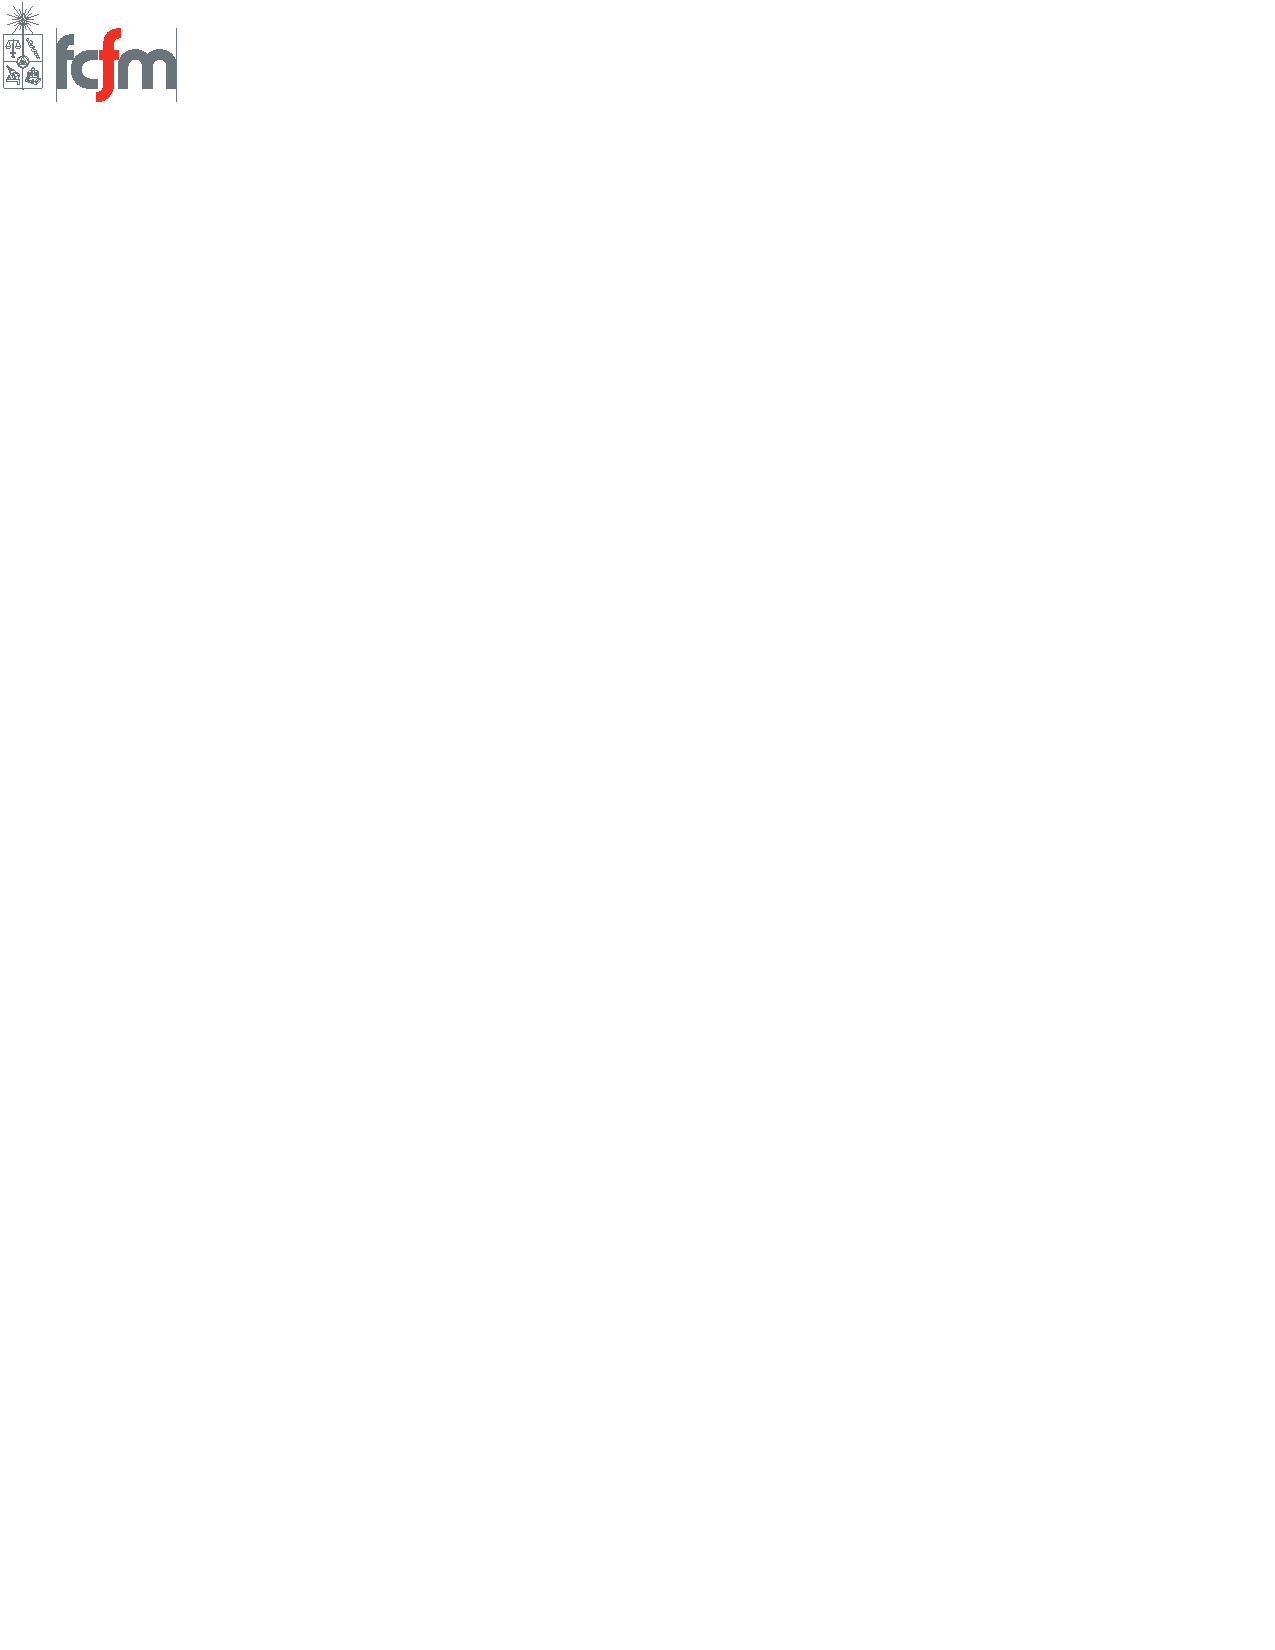
\includegraphics[scale=1.35]{departamentos/fcfm2}
	\end{wrapfigure}
	\hspace*{0.3cm}
	\noindent \textsc{\color{red} \hspace{-1.6cm} \departamentouniversidad} \\
	\hspace*{0.3cm}
	\noindent \textsc{\color{dgray} \hspace{-1.0cm} \nombrefacultad} \\
	\hspace*{0.3cm}
	\noindent \textsc{\color{dgray} \hspace{-1.0cm} \nombreuniversidad} \\
	\hspace*{0.3cm}
	\noindent \textsc{\color{dgray} \hspace{-1.0cm} \codigodelcurso \nombredelcurso}\\
	
	\begin{center}
		~ \\ [4.5cm]
		{\color{dgray} \Large \textsc{\temaatratar}}
		\rule{\linewidth}{.4mm} ~ \\ [0.4cm]
		{ \Huge \textup \bfseries \textsc{\titulodelinforme}} \\ [0.4cm]
		\rule{\linewidth}{.4mm} ~\\ [2.5cm]
	\end{center}
	\begin{minipage}{.5\textwidth}
		~
	\end{minipage}
	
	\vfill
	\tablaintegrantes
}{
\ifthenelse{\equal{\portraitstyle}{style4}}{
	\setpagemargincm{\pagemarginleft}{\pagemargintop}{\pagemarginright}{\pagemarginbottom}
	\pagestyle{empty}
	
\includegraphics[width=1.5cm]{departamentos/uchile2}
	\hspace{0cm}
	\begin{tabular}{l}
		\small \scshape{\MakeUppercase{\nombreuniversidad}} \\
		\small \scshape{\MakeUppercase{\nombrefacultad}} \\
		\small \scshape{\MakeUppercase{\departamentouniversidad}} \\
		\vspace*{1.25cm}\mbox{}
	\end{tabular}

	\vspace*{4 cm}
	\begin{center}
		\fontsize{8mm}{9mm} \selectfont 
		\titulodelinforme \\
		\vspace*{0.7cm}
		\footnotesize{\codigodelcurso\ - \nombredelcurso} \\
		\vspace*{3cm}
	\end{center}

	\vfill
	\tablaintegrantes
}{
	\throwbadconfigondoc{Estilo de portada incorrecto}{\portraitstyle}{style1,style2,style3,style4}}}}
}

% Añade una página en blanco al imprimir por las dos caras
\ifthenelse{\equal{\addemptypagetwosides}{true}}{
	\newpage
	\null
	\thispagestyle{empty}
	\renewcommand{\thepage}{}
	\newpage}{
}


% CONFIGURACIÓN DE PÁGINA Y ENCABEZADOS
% Template:     Informe/Reporte LaTeX
% Documento:    Configuración de página
% Versión:      4.3.6 (30/07/2017)
% Codificación: UTF-8
%
% Autor: Pablo Pizarro R.
%        Facultad de Ciencias Físicas y Matemáticas
%        Universidad de Chile
%        pablo.pizarro@ing.uchile.cl, ppizarror.com
%
% Manual template: [http://latex.ppizarror.com/Template-Informe/]
% Licencia MIT:    [https://opensource.org/licenses/MIT/]

% Numeración de páginas
\newpage
\ifthenelse{\equal{\romanpageuppercase}{true}}{
	\pagenumbering{Roman}
}{
	\pagenumbering{roman}
}
\setcounter{page}{1}
\setcounter{footnote}{1}

% Márgenes de páginas y tablas
\setpagemargincm{\pagemarginleft}{\pagemargintop}{\pagemarginright}{\pagemarginbottom}
\def\arraystretch{\tablepadding} % Se ajusta el padding de las tablas

% Se define el punto decimal
\ifthenelse{\equal{\pointdecimal}{true}}{
	\decimalpoint}{
}

% Definición de nombres de objetos
\renewcommand{\appendixname}{\nomltappendixsection} % Nom. del anexo en etiq. de título
\renewcommand{\appendixpagename}{\nameappendixsection} % Nombre del anexo en índice
\renewcommand{\appendixtocname}{\nameappendixsection} % Nombre del anexo en índice
\renewcommand{\contentsname}{\nomltcont}  % Nombre del índice
\renewcommand{\figurename}{\nomltwfigure} % Nombre de la leyenda de las fig.
\renewcommand{\listfigurename}{\nomltfigure} % Nombre del índice de figuras
\renewcommand{\listtablename}{\nomlttable} % Nombre del índice de tablas
\renewcommand{\lstlistingname}{\nomltwsrc} % Nombre leyenda del código fuente
\renewcommand{\lstlistlistingname}{\nomltsrc} % Nombre índice código fuente
\renewcommand{\refname}{\namereferences} % Nombre de las referencias
\renewcommand{\tablename}{\nomltwtable} % Nombre de la leyenda de tablas

% Numeración de objetos
\ifthenelse{\equal{\showsectiononcaption}{true}}{
	\counterwithin{equation}{section}   % Añade número de sección a las ecuaciones
	\counterwithin{figure}{section}     % Añade número de sección a las figuras
	\counterwithin{lstlisting}{section} % Añade número de sección a los códigos
	\counterwithin{table}{section}      % Añade número de sección a las tablas
}{}

% Se crean los header-footer
\ifthenelse{\equal{\hfstyle}{style1}}{
	\pagestyle{fancy} \fancyhf{}
	\fancyhead[L]{\nouppercase{\rightmark}}
	\fancyhead[R]{\small \rm \thepage}
	\fancyfoot[L]{\small \rm \textit{\titulodelinforme}}
	\fancyfoot[R]{\small \rm \textit{\codigodelcurso \nombredelcurso}}
	\renewcommand{\footrulewidth}{0.5pt}
	\renewcommand{\headrulewidth}{0.5pt}
	\renewcommand{\sectionmark}[1]{\markboth{#1}{}}
}{
\ifthenelse{\equal{\hfstyle}{style2}}{
	\pagestyle{fancy} \fancyhf{}
	\fancyfoot[C]{\thepage}
	\renewcommand{\headrulewidth}{0pt}
	\renewcommand{\footrulewidth}{0pt}
	\setlength{\headheight}{49pt}
}{
\ifthenelse{\equal{\hfstyle}{style3}}{
	\pagestyle{fancy} \fancyhf{}
	\fancyfoot[L]{\departamentouniversidad}
	\fancyfoot[C]{\thepage}
	\fancyfoot[R]{\nombreuniversidad}
	\renewcommand{\headrulewidth}{0pt}
	\renewcommand{\footrulewidth}{0pt}
	\setlength{\headheight}{49pt}
}{
\ifthenelse{\equal{\hfstyle}{style4}}{
	\pagestyle{fancy} \fancyhf{}
	\fancyfoot[R]{\thepage}
	\renewcommand{\headrulewidth}{0pt}
	\renewcommand{\footrulewidth}{0pt}
	\setlength{\headheight}{49pt}
}{
\ifthenelse{\equal{\hfstyle}{style5}}{
	\pagestyle{fancy} \fancyhf{}
	\fancyhead[L]{\codigodelcurso \nombredelcurso}
	\fancyhead[R]{\nouppercase{\rightmark}}
	\fancyfoot[L]{\departamentouniversidad, \nombreuniversidad}
	\fancyfoot[R]{\small \rm \thepage}
	\renewcommand{\footrulewidth}{0pt}
	\renewcommand{\headrulewidth}{0pt}
	\renewcommand{\sectionmark}[1]{\markboth{#1}{}}
}{
\ifthenelse{\equal{\hfstyle}{style6}}{
	\pagestyle{fancy} \fancyhf{}
	\fancyhead[L]{\nouppercase{\rightmark}}
	\fancyhead[R]{}
	\fancyfoot[C]{\small \rm \thepage}
	\renewcommand{\footrulewidth}{0pt}
	\renewcommand{\headrulewidth}{0.5pt}
	\renewcommand{\sectionmark}[1]{\markboth{#1}{}}
}{
	\throwbadconfigondoc{Estilo de header-footer incorrecto}{\hfstyle}{style1,style2,style3,style4,style5,style6}}}}}}
}

% Profundidad del índice
\setcounter{tocdepth}{\indexdepth} % Se ajusta la profundidad del índice



\chapter{Capítulo 1}

% RESUMEN O ABSTRACT
\begin{resumen}
	El trabajo fue realizado en el centro de investigación Web Intelligence Centre (WIC). Este consistió en el desarrollo del mapa de objectos claves del \textit{Proyecto AKORI}. \\ \\
	El \textit{Proyecto AKORI}, cuyo sigla en inglés es \textit{Advanced Kernel for Ocular Research and web Intelligence}, tiene como objetivo desarrollar una herramienta funcional que permita extrapolar el comportamiento de navegación para usuarios en un sitio web a partir de la extracción
de patrones desde datos analizados con técnicas de minería de datos, eye tracking y electroencefalografía. \\ \\
	El mapa de objetos claves realizado tiene la meta de mostrar de forma clara y precisa los objetos más relevantes del \textit{DOM} (\textit{Document Object Model}) cuando un usuario navega e ingresa a un sitio web. Con el objetivo de tener un indicador de los principales objetos que un usuario visualiza en los primeros milisegundos de ingresar a un sitio Web, facilitando así el trabajo de los diseñadores y desarrolladores que desean sitios Web más visitados y atractivos. El mapa de objetos claves fue realizado dos etapas, una etapa de migración y otra etapa de \textit{frontend}, siendo esencial la xetapa de migración para el desarrollo \textit{frontend}. \\ \\
	El trabajo realizado se encuentra actualmente intregado a la aplicación web oficial del \textit{Proyecto Akori} que se encuentra disponible en el sitio web. \\ \\
	En cuanto a aprendizajes obtenidos en el ámbito técnico se destaca el conocimiento adquirido del framework para desarrollo web \textit{Django}, el lenguaje script \textit{Javascritp} utilizado principalmente por el lado del cliente, y sistema de control de versiones Git. En cuanto otra habilidades aprendidas se destaca el trabajo en un equipo multidisciplinario.
\end{resumen}

% TABLA DE CONTENIDOS - ÍNDICE
% Template:     Informe/Reporte LaTeX
% Documento:    Índice
% Versión:      4.3.6 (30/07/2017)
% Codificación: UTF-8
%
% Autor: Pablo Pizarro R.
%        Facultad de Ciencias Físicas y Matemáticas
%        Universidad de Chile
%        pablo.pizarro@ing.uchile.cl, ppizarror.com
%
% Manual template: [http://latex.ppizarror.com/Template-Informe/]
% Licencia MIT:    [https://opensource.org/licenses/MIT/]

\ifthenelse{\equal{\showindex}{true}}{
	
	% Crea nueva página y establece estilo de títulos
	\newpage
	\tocloftpagestyle{fancy}
	\sectionfont{\color{\indextitlecolor} \fontsizetitlei \styletitlei \selectfont}
	
	% Configuración del punto en índice
	\ifthenelse{\equal{\showdotontitles}{true}}{
		\def\cftsecaftersnum {.}
		\def\cftsubsecaftersnum {.}
		\def\cftsubsubsecaftersnum {.}
		}{
	}

	% Configuración del punto en número de objetos
	\ifthenelse{\equal{\showdotonobjectindex}{true}}{
		\def\cftfigaftersnum {.}
		\def\cfttabaftersnum {.}
		\def\cftsubfigaftersnum {.}
		\def\cftlstlistingaftersnum {.}
		}{
	}

	% Configuración punto entre objeto y número de página
	\ifthenelse{\equal{\showdotpagenumindex}{true}}{}{
		\renewcommand{\cftdot}{}
	}
	
	% Índice de Contenidos
	\ifthenelse{\equal{\showindexofcontents}{true}}{\tableofcontents}{}
	
	% Lista de Figuras
	\iftotalfigures
		\ifthenelse{\equal{\showindexoffigures}{true}}{\listoffigures}{}
	\fi
	
	% Lista de Tablas
	\iftotaltables
		\ifthenelse{\equal{\showindexoftables}{true}}{\listoftables}{}
	\fi
	
	% Lista del Código Fuente
	\iftotallstlistings
		\ifthenelse{\equal{\showindexofcode}{true}}{\lstlistoflistings}{}
	\fi
	
	% Se añade una página en blanco
	\ifthenelse{\equal{\addemptypagetwosides}{true}}{
		\vfill
		\checkoddpage
		\ifoddpage
		\else
			\newpage
			\null
			\thispagestyle{empty}
			\newpage
			\addtocounter{page}{-1}
		\fi
	}{}

}{}
 % Índice, se puede borrar

% CONFIGURACIONES FINALES
% Template:     Informe/Reporte LaTeX
% Documento:    Archivo principal
% Versión:      4.3.6 (30/07/2017)
% Codificación: UTF-8
%
% Autor: Pablo Pizarro R.
%        Facultad de Ciencias Físicas y Matemáticas
%        Universidad de Chile
%        pablo.pizarro@ing.uchile.cl, ppizarror.com
%
% Manual template: [http://latex.ppizarror.com/Template-Informe/]
% Licencia MIT:    [https://opensource.org/licenses/MIT/]

% Se reestablecen headers y footers
\markboth{}{}
\newpage
\ifthenelse{\equal{\hfstyle}{style1}}{
	\fancyhead[L]{\nouppercase{\leftmark}}}{
}
\ifthenelse{\equal{\hfstyle}{style5}}{
	\fancyhead[R]{\nouppercase{\leftmark}}}{
}
\ifthenelse{\equal{\hfstyle}{style6}}{
	\fancyhead[L]{\nouppercase{\leftmark}}}{
}

% Se reestablece estilo de títulos
\sectionfont{\color{\titlecolor} \fontsizetitle \styletitle \selectfont}
\subsectionfont{\color{\subtitlecolor} \fontsizesubtitle \stylesubtitle \selectfont}
\subsubsectionfont{\color{\subsubtitlecolor} \fontsizesubsubtitle \stylesubsubtitle \selectfont}

% Se reestablecen números de página y secciones
\renewcommand{\thepage}{\arabic{page}}
\setcounter{page}{1}
\setcounter{section}{0}
\setcounter{footnote}{0}


% ======================= INICIO DEL DOCUMENTO =======================

% Template:     Informe/Reporte LaTeX
% Documento:    Archivo de ejemplo
% Versión:      4.3.6 (30/07/2017)
% Codificación: UTF-8
%
% Autor: Pablo Pizarro R.
%        Facultad de Ciencias Físicas y Matemáticas
%        Universidad de Chile
%        pablo.pizarro@ing.uchile.cl, ppizarror.com
%
% Manual template: [http://latex.ppizarror.com/Template-Informe/]
% Licencia MIT:    [https://opensource.org/licenses/MIT/]

% NUEVA SECCIÓN
% Las secciones se inician con \section, si se quiere una sección sin "número" se pueden usar las funciones \sectionanum (sección sin número) o la función \sectionanumnoi para crear el mismo título sin numerar y sin aparecer en el índice
\section{Introducción}
	
	% SUB-SECCIÓN
	% Las sub-secciones se inician con \subsection, si se quiere una sub-sección sin "número" se pueden usar las funciones \subsectionanum (nuevo subtítulo sin numeración) o la función \subsectionanumnoi para crear el mismo subtítulo sin numerar y sin aparecer en el índice
	\subsection{Lugar de Trabajo}
		
		\newpar{La prática profesional se realizó en el Web Intelligence Centre \cite{ref1}, en adelante WIC, es un centro de investigación depediente de la Facultad de Ciencias Físicas y Matemáticas de la Universidad de Chile, cuya misión es desarrollar investigación en el campo de Tecnologías de Información creando soluciones para abordar problemas complejos de ingeniería utilizando herramientas basadas en la Web de las Cosas. Se encuentra ubicado en Beaucheff \#851, Santiago, Chile. El trabajo se realizó de forma presencial en las instalaciones del centro, entre el 3 al 31 de Enero de 2017.}
		

	\subsection{Grupo de trabajo}
	
		\newpar{En el WIC trabajan investigadores de tiempo completo, desarrolladores con experiencia, profesionales del área de la salud debido a que muchos de sus proyectos son en conjunto con la Facultad de Medicina, alumnos de pregrado que pueden ser memorista sobre algún tema de investigación o trabajadores part-time y estudiantes de magister del Departamento de Ingeniería Industrial. En particular en la oficina donde se realizó el trabajo era usada regularmente por 6 personas, de los cuales había un investigador, dos memorista, un ingeniero de proyectos y otro practicante que también trabajó en el \textit{Proyecto AKORI}, que es dirigido por el Ingeniero de Proyecto, Felipe Vera, quien fue el tutor del practicante (pero no se encontraba en la misma oficina).}
\newpage
\subsection{Equipos y Software}	
	
		\subsubsection{Software}
			\newpar{El software utilizado para desarrollar el trabajo fue \textit{Python} como lenguaje de programación (a través del IDLE Pycharm proporcionado por JetBrains \cite{ref2}), el framework para aplicaciones Web Python, \textit{Django}, \textit{Javascript} y \textit{AJAX} para la creación de páginas web dinámicas, \textit{Git} para el manejo de control de versiones, el navegador sin interfaz gráfico (conocido como headless browser), PhantomJS, el entorno de pruebas software para aplicaciones web, Selenium, dos bibliotecas de Python, una para edición de imágenes, Python Imaging Library, y otra para la generación de un mapa de colores, Matplotlib, y el sistema operativo Ubuntu. Además cabe descatar del aplicación del \textit{Proyecto AKORI} en la cual se trabajo. A continuación se presenta una breve descripción de los elementos más relevantes para el desarrollo y compresión del trabajo realizado:}
			\begin{enumerate}
				\item \textbf{Python}: Es un lenguaje de programación interpretado cuya filosofía 
				hace hincapié en una sintaxis que favorezca un código legible. Se trata de un 
				lenguaje de programación multiparadigma, ya que soporta orientación a objetos, 
				progrmación imperativa y, en menor medida, programación funcional. En el contexto 
				del trabajo Python sirvió como lenguaje de programación por el lado del servidor 
				para la aplicación web que actualmente funciona como prototipo al \textit{Proyecto AKORI}. 
				\item \textbf{Django}: Es un framework de desarrollo web de código abierto (\textit{open source}), escrito en \textit{Python} que respeta el patrón de diseño conocido como 
				Modelo-Vista-Controlador (MCV), que en pocas palabras separa los componentes más 
				importantes de una aplicación es tres grandes grupos, el modelo donde descansan los
				datos de la aplicación (Base de Datos), la vista que se encarga de todo el aspecto 
				visual de una aplicación, y los controladores que ejecutan toda la lógica de
				funcionamiento. \\ 
				En el caso de \textit{Django} tiene la perculiaridad que las vistas reciben el 
				nombre templates (encargados del \textit{fontend} de la aplicación) y los 
				controladores se llaman vistas (Views en inglés y encargadas del \textit{backend}). 	
				Para el trabajo realizado fue necesario tomar la aplicación desarrollada, anadir
				cambios en los templates y agregar algunas funciones a las vistas para controlar 
				la lógica de la mapa de objetos que en las próximas secciones serán explicadas en 
				detalle.
				\item \textbf{Javascript} y \textbf{AJAX}: Es un lenguaje de programación que 
				es utilizado para la creación de páginas web de dinámicas por el lado del cliente
				en una aplicación web. \textit{AJAX} es una extensión a la funcionalidad de 
				\textit{Javascript} que hace llamadas asincronas al servidor web obteniendo 
				información sin recargar las página por completo. Dentro del trabajo de prática
				fueron utilizados para obtener el input de datos para el despliegue del mapa de 
				objetos sin recargar toda la aplicación en la consulta. 
				\item \textbf{PhantomJS}: Es un navegador sin interfaz gráfica que sirve para 
				realizar pruebas a una aplicación que se encuentra en fase de desarrollo. Fue 
				utilizado para realizar web scrapping, término que describe la recolección de 
				información a través de la Web usando programas automatizados.
				\item \textbf{Selenium}: Es un entorno de pruebas de software para aplicaciones 
				basadas en la web. Se usó para realizar el web scrapping junto a PhantomJs sobre
				los distintas sitios web que fueron testeados.
			\end{enumerate}
	\subsubsection{\textit{Proyecto AKORI}}
	
		\newpar{Para contextualizar de mayor forma el trabajo de práctica realizado a continuación 
		se explicará brevemente que es el \textit{Proyeto AKORI} y cuál es su meta a seguir. }
		
	\subsubsection{Equipo}
	
		\newpar{En cuanto a los equipos computacionales, el centro provee tanto equipos
		estacionarios como portátiles para aquellos que encuentran trabajando e investigando, 
		sin embargo para los prácticantes y memoristas deben llevar sus equipos personales 
		para desarrollar sus labores. En particular la prática realizada solo fue necesario un
		equipo portátil para programar el mapa de objetos.}

	\subsection{Situación Previa}
% NUEVA SECCIÓN
\newpage
\section{Conclusiones}
 	\newpar{Los resultados del trabajo presentado en este informe fueron considerados por el tutor
 	de práctica como satifactorios, siendo estos puestos en producción al poco tiempo de finalizada la 			práctica, los cuales pueden ser apreciados en la página oficial del \textit{Proyecto AKORI} 			\cite{ref3}. Además gracias a la programación hecha por el prácticante cuando se ingresa la url del sitio web a analizar no solo es posible generar un mapa de los objetos más relevantes encerrados por rectangulos, sino que existe un mapa en escala de intensidad de colores de los objetos web más a los menos vistos por un usuario (en el sitio web que se está analizando), cambiando la escala en cuatro colores rojo, naranjo, azul y verde. \\ \\ Respecto al futuro de la aplicación
 	hay que destacar que aún se encuentra trabajando en ella realizando actulizaciones para mejorar su llegada al público o a los posible clientes (si llega a comercializarse) en términos de 
 	visualizaciones que le provean más y mejor información al usuario sobre el sitio web a analizar, 
 	en particular se seguirá trabajando en las secciones modificadas y agregadas por el practicante,
 	en miras de mejorar la performance de las visualizaciones de los elementos más vistos dentro 
 	del DOM en el mapa de objetos mediante optimizaciones en la extracción de datos y algoritmos
 	de búsqueda de objetos web más eficientes. \\ \\ Dentro del aprendizaje obtenido en el proceso
 	de práctica se destacan a nivel técnico el aprendizaje del framework \textit{Django} para el desarrollo web y sus elementos específicos como vistas, modelos, templates. También el aprendizaje 
 	de \textit{Javascritp} es especialmente el uso de \textit{AJAX} para el despligue del mapa de
 	objetos sin actualizar la página completa y \textit{Git} para el manejo de control de versiones.
 	Otro punto no menos importante dentro del aprendizajes de todas las tecnologías fue lo 
 	primordial que es leer la documentación antes de utilizar cualquier tecnología ya que 
 	simplifica mucho el tiempo de aprendizaje. Dentro de otros aspectos se aprendió sobre el
 	trabajo en equipo, la importancia de mantener constantemente comunicación para realizar un 
 	buen trabajo en particular cuando se trabaja en un equipo multidisciplinario. El practicante
 	estuvo en constante contacto con algunos investigadores y el con encargado para obtener un 
 	mapa de objeto acorde a los requerimientos y entendible para cualquier usuario use la 
 	plataforma del \textit{Proyecto AKORI}. Finalmente queda destacar el aprendizaje de documentar
 	bien el código hecho para que sea fácil de entender y extender a medida que el proyecto crece, 
 	y además de contar con buen diseño en el código muchas veces esto puede resultar fácil, pero
 	en la práctica puede ser determinante la contuinidad de una aplicación robusta que pueda seguir
 	creciendo y no empezar un sistema que prácticamente hará lo mismo desde 0.}

\newpage
\section{Aquí un nuevo tema}
	
	% SUB-SECCIÓN
	\subsection{Haciendo informes como un profesional}
		
		% Se inserta una imagen flotante en la izquierda del documento con \insertimageleft, al igual que las demás funciones, el primer parámetro es opcional, luego viene la ubicación de la imagen, seguido de la escala y por último su leyenda. Para insertar una imagen flotante en la derecha se utiliza \insertimageright usando los mismos parámetros
		\insertimageleft[\label{img:imagen-izquierda}]{ejemplos/test-image-wrap}{0.3}{Apolo flotando a la izquierda.}
		
		\lipsum[1]

		% Párrafos con \newp, lipsum por defecto no añade un párrafo nuevo
		\newp \lipsum[115]
		\newp \lipsum[2]
		
		% Agrega una ecuación con leyendas
		\insertequationcaptioned[\label{eqn:formulasinsentido}]{\int_{a}^{b} f(x) \dd{x} = \fracnpartial{f(x)}{x}{\eta} \cdotp \textstyle \sum_{x=a}^{b} f(x)\cancelto{1+\frac{\epsilon}{k}}{(1+\Delta x)}}{Ecuación sin sentido.}
		
		% Aquí no es necesario usar \newp dado que todas las funciones \insert... añaden un párrafo nuevo por defecto
		\lipsum[115]
		
		% Párrafos con \newp, lipsum por defecto no añade un párrafo nuevo
		\newp \lipsum[4]
		
	% Inserta un subtítulo sin número
	\subsection{Otros párrafos más normales}
	
		% Párrafos con lipsum
		\lipsum[7]
		
		\newp \lipsum[2]
		
		% Se inserta una ecuación larga con el entorno gathered (1 solo número de ecuación)
		\insertgathered[\label{eqn:eqn-larga}]{
			\lpow{\Lambda}{f} = \frac{L\cdot f}{W} \cdot \frac{\pow{\lpow{Q}{e}}{2}}{8 \pow{\pi}{2} \pow{W}{4} g} + \sum_{i=1}^{l} \frac{f \cdot \big( M - d\big)}{l \cdot W} \cdot \frac{\pow{\big(\lpow{Q}{e}- i\cdot Q\big)}{2}}{8 \pow{\pi}{2} \pow{W}{4} g}\\
			Q_e = 2.5Q \cdot \int_{0}^{e} V(x) \dd{x}
		}
	
		% Nuevo párrafo
		\lipsum[4]
		
		% Se inserta un multicols, con esto se pueden escribir en varias columnas
		\begin{multicols}{2}
			
			% Párrafo 1
			\lipsum[4]
			
			% Ecuación encerrada en una caja
			\insertequation[]{ \boxed{f(x) = \fracdpartial{u}{t}} }
			
			% Párrafo 2 del multicols
			\lipsum[1]
			
		\end{multicols}
		
	% SUB-SECCIÓN
	\subsection{Ejemplos de inserción de código fuente}
		
		A continuación se presenta un ejemplo de inserción de código fuente en Python\footnote{El mejor lenguaje del mundo.} (Código \ref{codigo-python}), Java (Código \ref{codigo-java}) y Matlab (Código \ref{codigo-matlab}) utilizando el entorno \texttt{lstlisting}:
		
% Se define el lenguaje del código, cuidado: Los códigos en LaTeX son sensibles a las tabulaciones y espacios en blanco
\begin{lstlisting}[style=Python, caption={Ejemplo en Python.\label{codigo-python}}]
import numpy as np

def incmatrix(genl1, genl2):
	m = len(genl1)
	n = len(genl2)
	M = None # Comentario 1
	VT = np.zeros((n*m, 1), int) # Comentario 2
\end{lstlisting}

\begin{lstlisting}[style=Java, caption={Ejemplo en Java.\label{codigo-java}}]
import java.io.IOException; 
import javax.servlet.*;

// Hola mundo
public class Hola extends GenericServlet {
	public void service(ServletRequest request, ServletResponse response)
	throws ServletException, IOException{
		response.setContentType("text/html");
		PrintWriter pw = response.getWriter();
		pw.println("Hola, mundo!");
		pw.close();
	}
}
\end{lstlisting}

\begin{lstlisting}[style=Matlab, caption={Ejemplo en Matlab.\label{codigo-matlab}}]
% Se crea gráfico
f = figure(1); hold on; movegui(f, 'center');
xlabel('td/Tn'); ylabel('FAD=Umax/Uf0');
title('Espectro de pulso de desplazamiento');

for j = 1:length(BETA)
	fad = ones(1, NDATOS); % Arreglo para el FAD, uno para cada r (o td/Tn)
	
	% Se crea el espectro de respuesta máximo para cada par de beta/r
	for i = 1:NDATOS
		[t, u_t, ~, ~] = main(BETA(j), r(i), M, K, F0, 0);
		fad(i) = max(abs(u_t)) / uf0;
	end
	mx = find(fad == max(fad(:)));
	fprintf('BETA=%.2f, MAX: FAD=%.3f, TD/TN=%.3f\n', BETA(j), fad(mx), tdtn(mx));
	plot(tdtn, fad, 'DisplayName', strcat('\beta=', sprintf('%.2f', BETA(j))));
end
\end{lstlisting}


% NUEVA SECCIÓN
% Inserta una sección sin número
\section{Más ejemplos}
	
	% Inserta un subtítulo sin número
	\subsection{Listas y Enumeraciones}
		
		Hacer listas enumeradas con \LaTeX\ es muy fácil \footnote{También puedes revisar el manual de las enumeraciones en \url{http://www.texnia.com/archive/enumitem.pdf}}, para eso debes usar el comando \texttt{\textbackslash begin\{enumerate\}}, cada elemento empieza por \texttt{\textbackslash item}, resultando:
		
		\begin{enumerate}
			\item Ítem 1
			\item Abracadabra
			\item Manzanas
		\end{enumerate}
		
		También se puede cambiar el tipo de enumeración, se pueden usar letras, números romanos, entre otros. Esto se logra cambiando el \textbf{label} del objeto \texttt{enumerate}. A continuación se muestra un ejemplo usando letras con el estilo \texttt{\textbackslash alph} \footnote{Con \texttt{\textbackslash Alph} las letras aparecen en mayúscula}, números romanos con \texttt{\textbackslash roman} \footnote{Con \texttt{\textbackslash Roman} los números romanos salen en mayúscula} o números griegos con \texttt{\textbackslash greek} \footnote{Una característica propia del template, con \texttt{\textbackslash Greek} las letras griegas están escritas en mayúscula}:
		
		\begin{multicols}{3}
			\begin{enumerate}[label=\alph*) ,font=\bfseries] % Fuente en negrita
				\item Peras
				\item Manzanas
				\item Naranjas
			\end{enumerate}
			
			\begin{enumerate}[label=\greek*) ]
				\item Matemáticas
				\item Lenguaje
				\item Filosofía
			\end{enumerate}
		
			\begin{enumerate}[label=\roman*) ]
				\item Rojo
				\item Café
				\item Morado
			\end{enumerate}
		\end{multicols}
		
		Para hacer listas sin numerar con \LaTeX\ hay que usar el comando \texttt{\textbackslash begin\{itemize\}}, cada elemento empieza por \texttt{\textbackslash item}, resultando:
		
		\begin{multicols}{3}
			\begin{itemize}[label={--}]
				\item Peras
				\item Manzanas
				\item Naranjas
			\end{itemize}
			
			\begin{enumerate}[label={*}]
				\item Rojo
				\item Café
				\item Morado
			\end{enumerate}
			
			\begin{itemize}
				\item Árboles
				\item Pasto
				\item Flores
			\end{itemize}
		\end{multicols}
		
	% Inserta un subtítulo sin número
	\subsection{Otros}
		
		Recuerda revisar el manual de todas las funciones de este template visitando el siguiente link: \url{http://ppizarror.com/Template-Informe/}. Además si necesitas una ayuda muy específica sobre el template me puedes enviar un correo a \insertemail{pablo.pizarro@ing.uchile.cl}.

% ANEXO
\newpage
\begin{anexo}
	\section{Cálculos realizados}
	
		\lipsum[69]
		
		% Imagen, se numerará automáticamente con la letra del anexo
		\insertimage[\label{img:anexo-2}]{ejemplos/test-image.png}{scale=0.15}{Imagen en anexo.}
		
		\lipsum[10]
		
		% Tablas
		\begin{table}[htbp]
			\centering
			\caption{Tabla de cálculo.}
			\begin{tabular}{ccc}
				\hline
				\textbf{Elemento} & $\epsilon_i$ & \boldmath{}\textbf{Valor}\unboldmath{} \bigstrut\\
				\hline
				A     & 10    & 3,14$\pi$ \bigstrut[t]\\
				B     & 20    & 6 \\
				C     & 30    & 7 \\
				\end{tabular}
			\label{tab:anexo-1}
		\end{table}
	
	\newpage
	\section{Más cálculos}
	
		% Párrafo
		\lipsum[1]\newp\lipsum[4]
		
		% Tabla de encuestas
		\begin{table}[htbp]
			\centering
			\caption{Resultados encuesta.}
			\begin{tabular}{ccc}
				\hline
				\textbf{Herramienta} & \textbf{Nota} & \textbf{Recomendado} \bigstrut\\
				\hline
				Word  & 0\%   & No $\frownie$\\
				\LaTeX & 100\% & Si $\checkmark$ \\
			\end{tabular}
			\label{tab:anexo-2}
		\end{table}
		
\end{anexo}

% REFERENCIAS (ESTILO BIBTEX)
\newpage % Salto de página
\begin{references}
	\bibitem{ref1}
	\textit{Sitio Web del WIC}
	\url{http://www.wic.uchile.cl}
	
	\bibitem{ref2}
	\textit{PyCharm IDLE}
	\url{https://www.jetbrains.com/pycharm/}
	
	\bibitem{ref3}
	\textit{Página Oficial del Proyecto AKORI} 
	\url{https://www.akori-project.cl}
\end{references}
 % Ejemplo, se puede borrar

% FIN DEL DOCUMENTO
\end{document}
